\documentclass[handout,compress]{beamer}

\usetheme[block=fill]{metropolis}

\usepackage{graphicx} % Allows including images
\usepackage{amsmath,amsfonts,amsthm,amssymb}
\usepackage{color}
\usepackage{xcolor,cancel}
%\setitemize{label=\usebeamerfont*{itemize item}%
%	\usebeamercolor[fg]{itemize item}
%	\usebeamertemplate{itemize item}}
\definecolor{mDarkBrown}{HTML}{604c38}
\definecolor{mDarkTeal}{HTML}{23373b}
\definecolor{mLightBrown}{HTML}{EB811B}
\definecolor{mMediumBrown}{HTML}{C87A2F}
\definecolor{mygreen}{HTML}{98C2B9}
\definecolor{myyellow}{HTML}{DFD79C}
\definecolor{myblue}{HTML}{8CA7CC}
\definecolor{kern}{HTML}{8CC2B7}

\usepackage{float}
\usepackage{framed}
\usepackage{epsfig}
\usepackage{graphicx}
\usepackage{subcaption}
\usepackage{ulem}
\usepackage{hhline}
\usepackage{multirow}
\usepackage{comment}   
\usepackage{bbm}
\usepackage{tikz}   
\usepackage{ulem}
\def\Put(#1,#2)#3{\leavevmode\makebox(0,0){\put(#1,#2){#3}}}
\newcommand*\mystrut[1]{\vrule width0pt height0pt depth#1\relax}
\newcommand{\eqdef}{\mathbin{\stackrel{\rm def}{=}}}


\newcommand{\bs}[1]{\boldsymbol{#1}}
\newcommand{\bv}[1]{\mathbf{#1}}
\newcommand{\R}{\mathbb{R}}
\newcommand{\E}{\mathbb{E}}

\DeclareMathOperator*{\argmin}{arg\,min}
\DeclareMathOperator*{\argmax}{arg\,max}
\DeclareMathOperator{\nnz}{nnz}
\DeclareMathOperator{\Var}{Var}
\DeclareMathOperator{\sinc}{sinc}
\DeclareMathOperator{\mv}{mv}
\DeclareMathOperator{\sgn}{sgn}
\DeclareMathOperator{\step}{step}
\DeclareMathOperator{\gap}{gap}
\DeclareMathOperator{\poly}{poly}
\DeclareMathOperator{\tr}{tr}
\DeclareMathOperator{\orth}{orth}
\newcommand{\norm}[1]{\|#1\|}
\captionsetup[subfigure]{labelformat=empty}
\captionsetup[figure]{labelformat=empty}
\DeclareMathOperator*{\lmin}{\lambda_{min}}
\DeclareMathOperator*{\lmax}{\lambda_{max}}

\newcommand{\specialcell}[2][c]{%
	\begin{tabular}[#1]{@{}c@{}}#2\end{tabular}}
\newcommand{\specialcellleft}[2][c]{%
	\begin{tabular}[#1]{@{}l@{}}#2\end{tabular}
}

\usepackage{tabstackengine}
\stackMath

\newtheorem{claim}[theorem]{Claim}


%----------------------------------------------------------------------------------------
%	TITLE PAGE
%----------------------------------------------------------------------------------------

\title{CS-UY 4563: Lecture 21 \\ Auto-encoders, Principal Component Analysis}
\author{NYU Tandon School of Engineering, Prof. Christopher Musco}
\date{}

\begin{document}
	
	\begin{frame}
		\titlepage 
	\end{frame}
	
	\metroset{titleformat=smallcaps}
	
	\begin{frame}
		\small
		\frametitle{course logistics}
		\begin{itemize}
			\item Next weeks should be focused on project work! Final report due \textbf{5/11}. 
			\item I am still working through proposals. If you feel blocked/need my input to move forward on project, please email or come to office hours.
			\item Each group will give a \textbf{5 minute presentation} in class on \textbf{5/6} or \textbf{5/11}. Link for signing up for a slot is on the course webpage. 
			\item Details on expectations for presentation will be released soon.    
		\end{itemize}
	\end{frame}

\begin{frame}
	\frametitle{transfer learning}
	Machine learning algorithms like neural networks \emph{learn high level features}.
	\begin{center}
		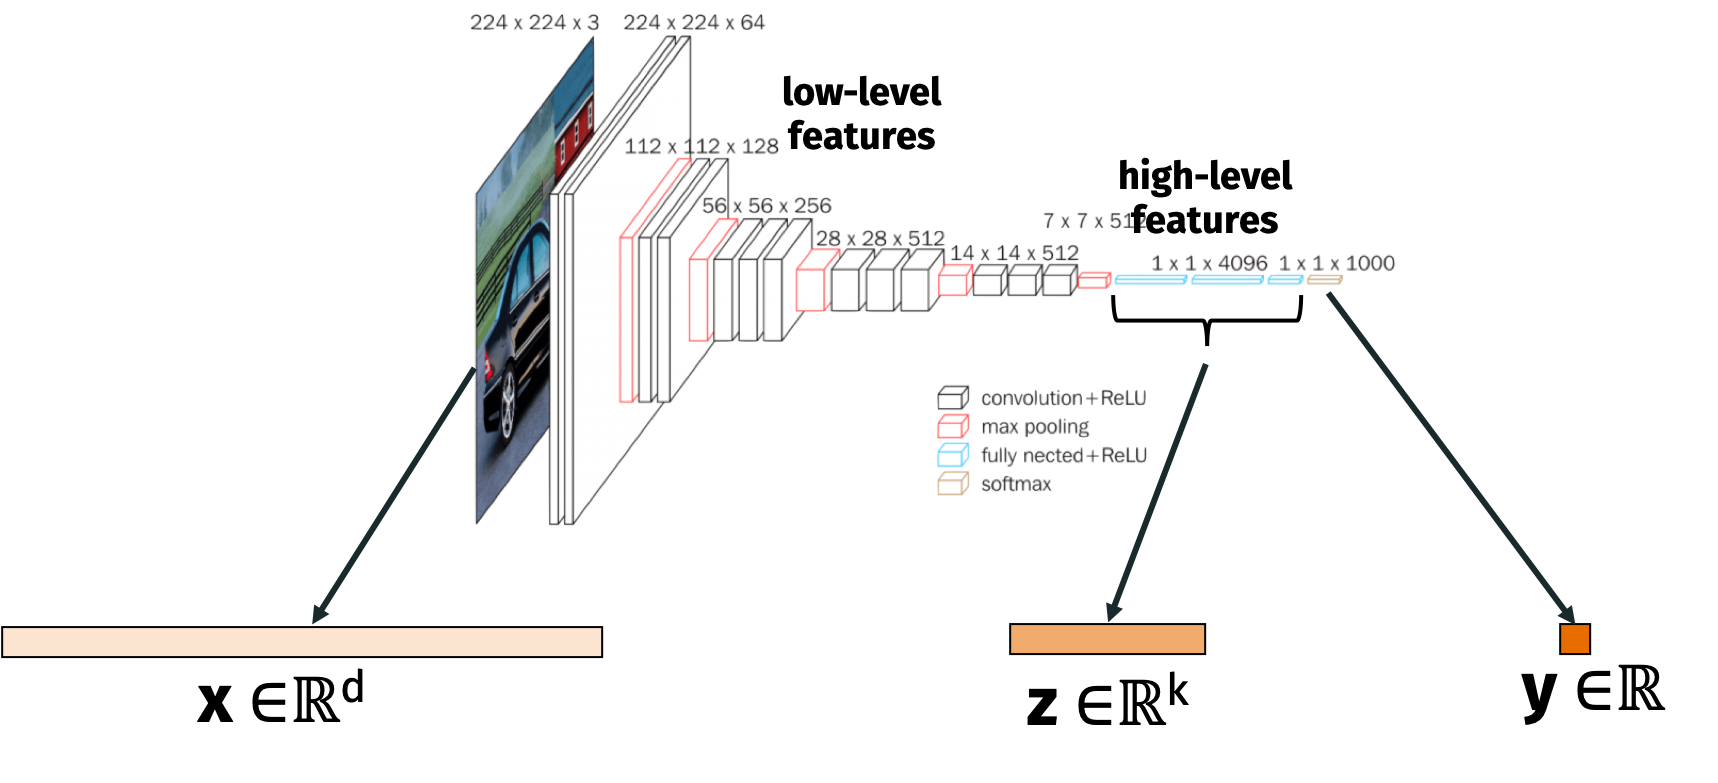
\includegraphics[width=\textwidth]{transfer_abstract.png}
	\end{center}
These features are useful for other tasks that the network was not trained specifically to solve.
\end{frame}

\begin{frame}
	\frametitle{autoencoder}
	\small
	\textbf{Idea behind \emph{autoencoders}}: If you have limited labeled data, make the inputs the targets. Learn to reconstruct input data and extract high-level features along the way.
	\begin{center}
		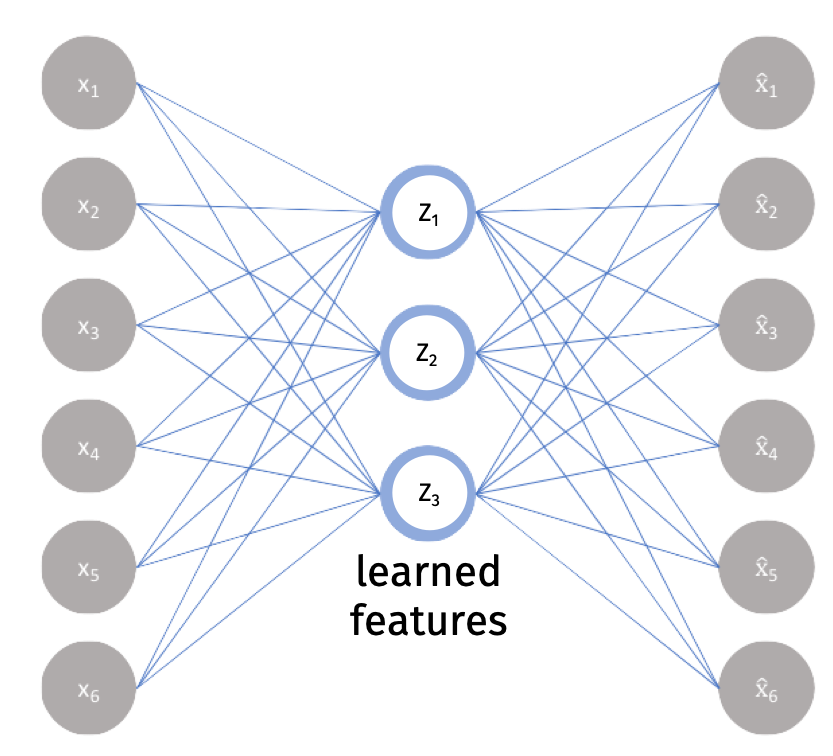
\includegraphics[width=.4\textwidth]{bottleneck.png} \hspace{2em}
		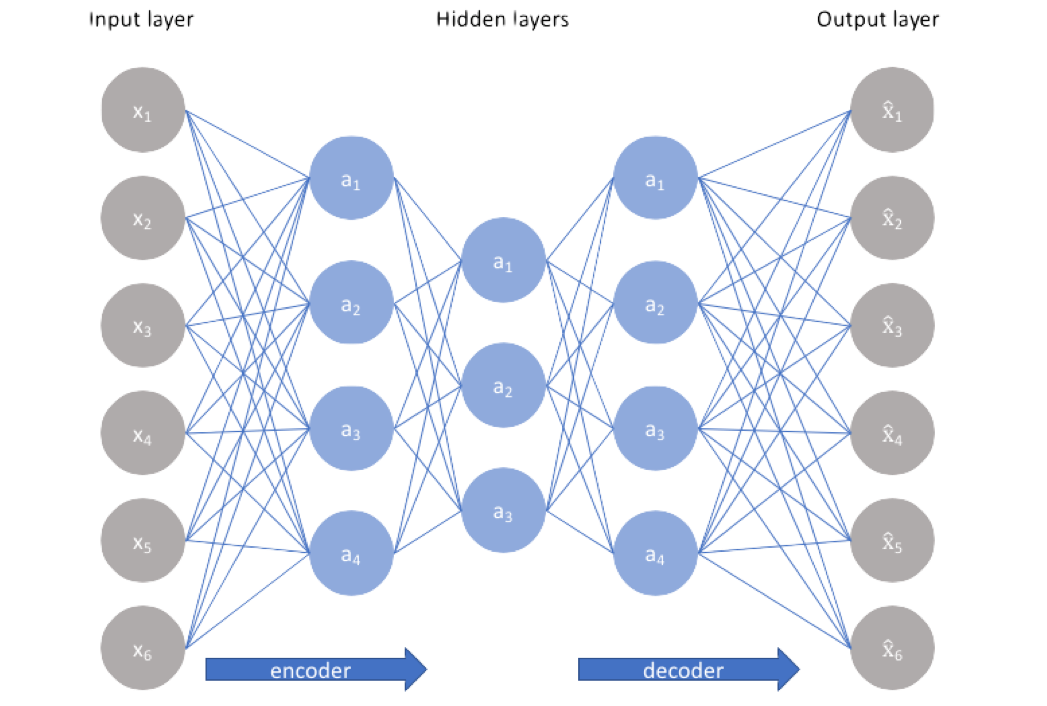
\includegraphics[width=.4\textwidth]{deeper_bottleneck.png}
		
		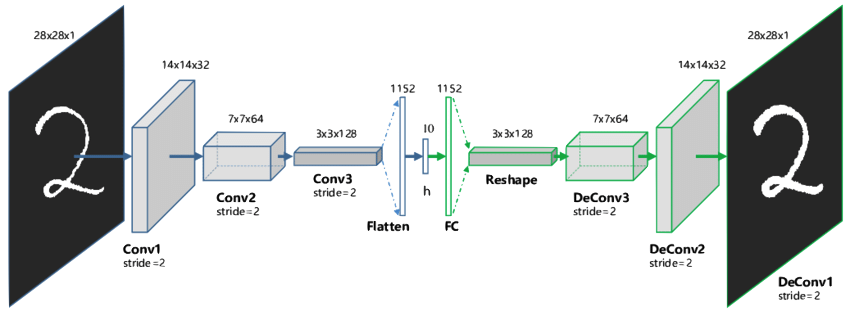
\includegraphics[width=.6\textwidth]{conv_autoencode.png}
	\end{center}	
\end{frame}

\begin{frame}
	\frametitle{autoencoder}
	
	\textbf{Encoder:} $e: \R^d \rightarrow \R^k$
	
	\textbf{Decoder:} $d: \R^k \rightarrow \R^d$
	\begin{align*}
		f(\vec{x}) = e(d(x))
	\end{align*}
	\begin{center}
		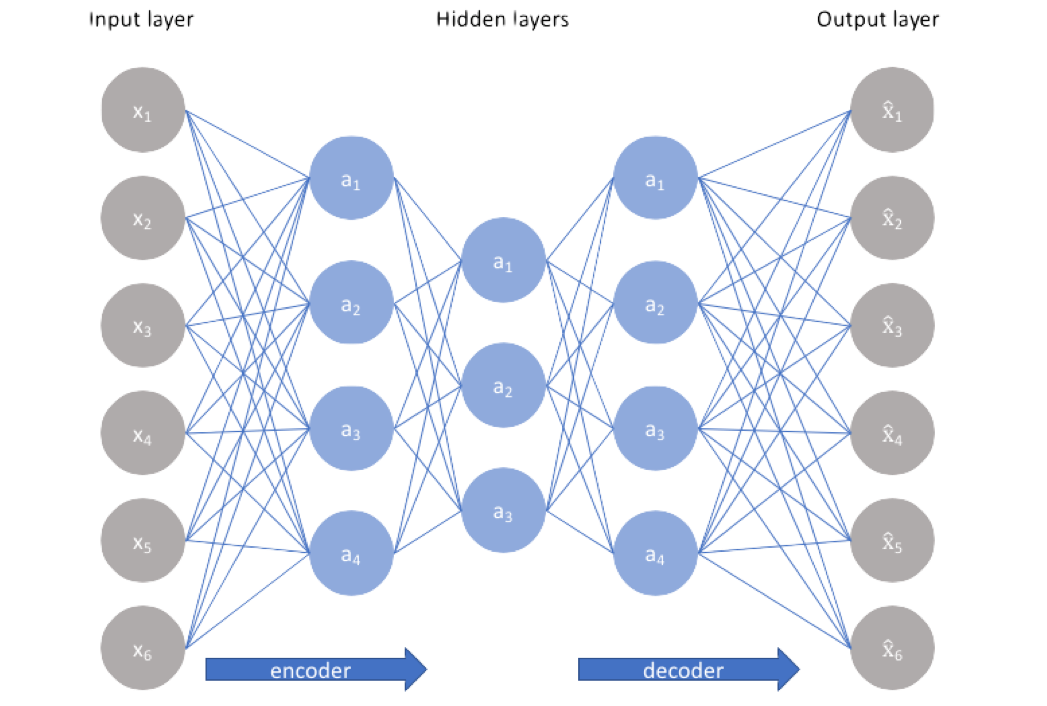
\includegraphics[width=.5\textwidth]{deeper_bottleneck.png}
		
		The number of learned features $k$ is typically $\ll d$. 
	\end{center}
	
\end{frame}

\begin{frame}
	\frametitle{autoencoder reconstruction}\small
	\textbf{Example image reconstructions from autoencoder:}
	\begin{center}
		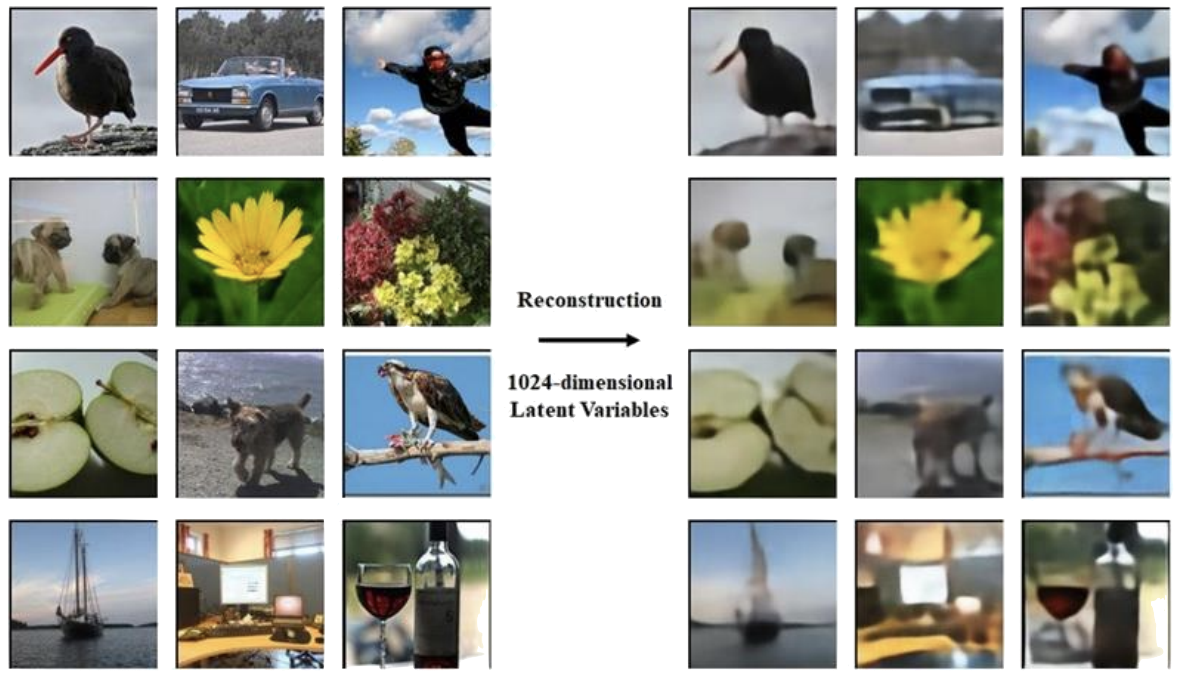
\includegraphics[width=.8\textwidth]{reconstruction.png}
		
		\tiny{\url{https://www.biorxiv.org/content/10.1101/214247v1.full.pdf}}
	\end{center}
	\textbf{Input parameters:} $d = 49152$.\vspace{-.5em}
	
	\textbf{Bottleneck ``latent" parameters:} $k = 1024$.  
\end{frame}


\begin{frame}
	\frametitle{autoencoders for feature extraction}
	Autoencoders also have \emph{many other applications} besides feature extraction.
	\begin{itemize}
		\item Learned image compression.
		\item Denoising and in-painting.
		\item Image synthesis.
	\end{itemize}
\end{frame}

\begin{frame}
	\frametitle{autoencoders for data compression}
	Due to their bottleneck design, autoencoders perform \textbf{dimensionality reduction} and thus data compression. 
	\begin{center}
		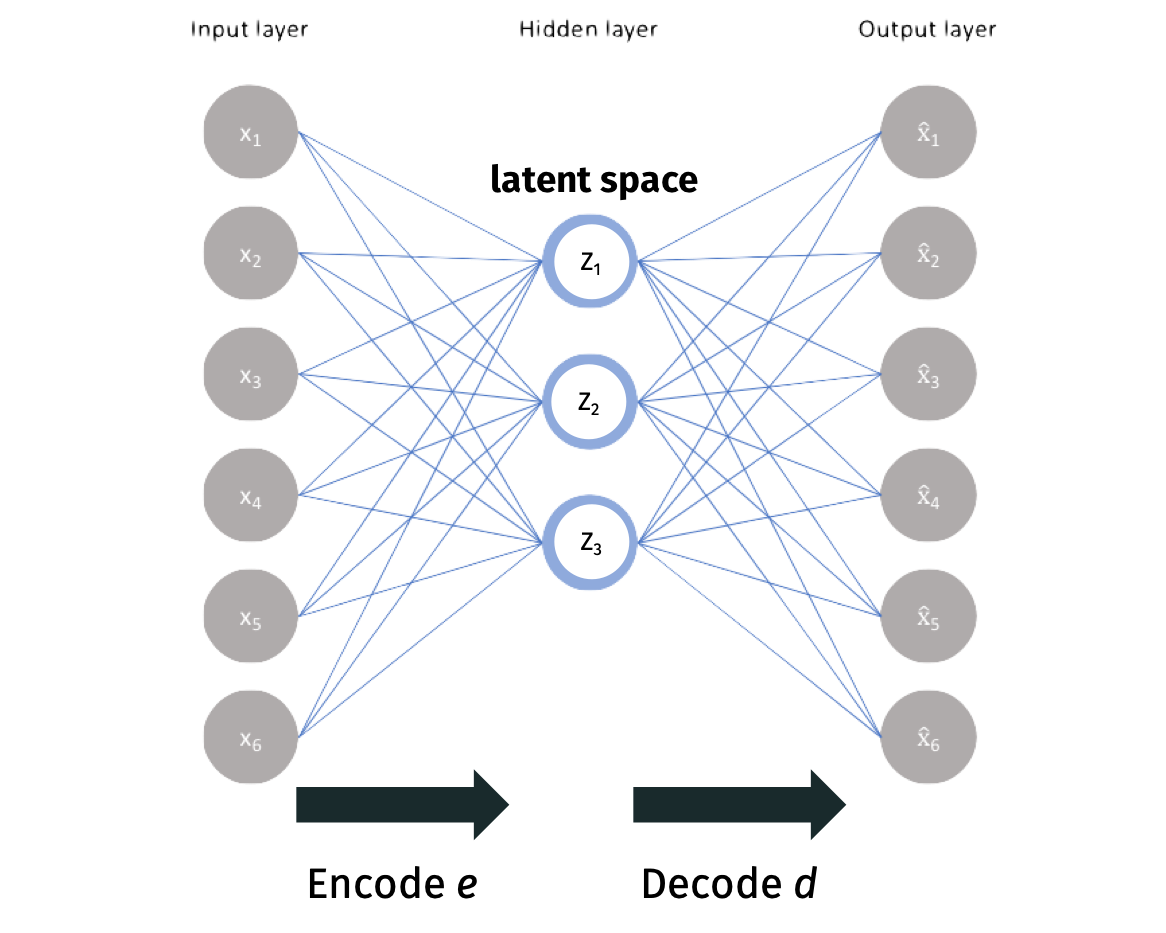
\includegraphics[width=.5\textwidth]{labeled_bottleneck.png}
	\end{center}
Given input $\vec{x}$, we can completely recover $f(\vec{x})$ from $\vec{z} = e(\vec{x})$. $\vec{z}$ typically has many fewer dimensions than $\vec{x}$ and for a typical $f(\vec{x})$ will closely approximate $\vec{x}$.  
\end{frame}

\begin{frame}
	\frametitle{autoencoders for image compression}
	\small
	The best lossy compression algorithms are tailor made for specific types of data:\vspace{-.5em}
	\begin{itemize}
		\item JPEG 2000 for images
		\item MP3 for digital audio.
		\item MPEG-4 for video.
	\end{itemize}\vspace{-.5em}
	All of these algorithms take advantage of specific structure in these data sets. E.g. JPEG  assumes images are locally ``smooth".
	\begin{center}
%		\includegraphics*[width=.3\textwidth]{bwnyu.png}\hspace{4em} \includegraphics*[width=.3\textwidth]{scrambled_nyu.png}
	\end{center}
\end{frame}

\begin{frame}
	\frametitle{autoencoders for image compression}
	\small
	With enough input data, autoencoders can be trained to find this structure on their own.
	\begin{center}
%		\includegraphics*[width=.4\textwidth]{compress1.png}\hspace{2em} \includegraphics*[width=.4\textwidth]{compress2.png}
		
		\tiny{``End-to-end optimized image compression'', Ball\'{e}, Laparra, Simoncelli}
	\end{center}
	 Need to be careful about how you choose loss function, design the network, etc. but can lead to much better image compression than ``hand-designed" algorithms like JPEG.
\end{frame}

\begin{frame}
	\frametitle{autoencoders for data restoration}
	\small
	\vspace{-1.5em}
	\begin{center}
		\includegraphics*[width=.6\textwidth]{resto.png}
	\end{center}
\vspace{-2em}
	Train autoencoder on \emph{uncorrupted} data. Pass corrupted data $\vec{x}$ through autoencoder and return $f(\vec{x})$ as repaired result.\footnote{Works much better if trained on corrupted data. More on this later.}
\end{frame}

\begin{frame}
	\frametitle{autoencoders learn compressed representations}
	\small
	\begin{center}
	\textbf{Why does this work?}
	
	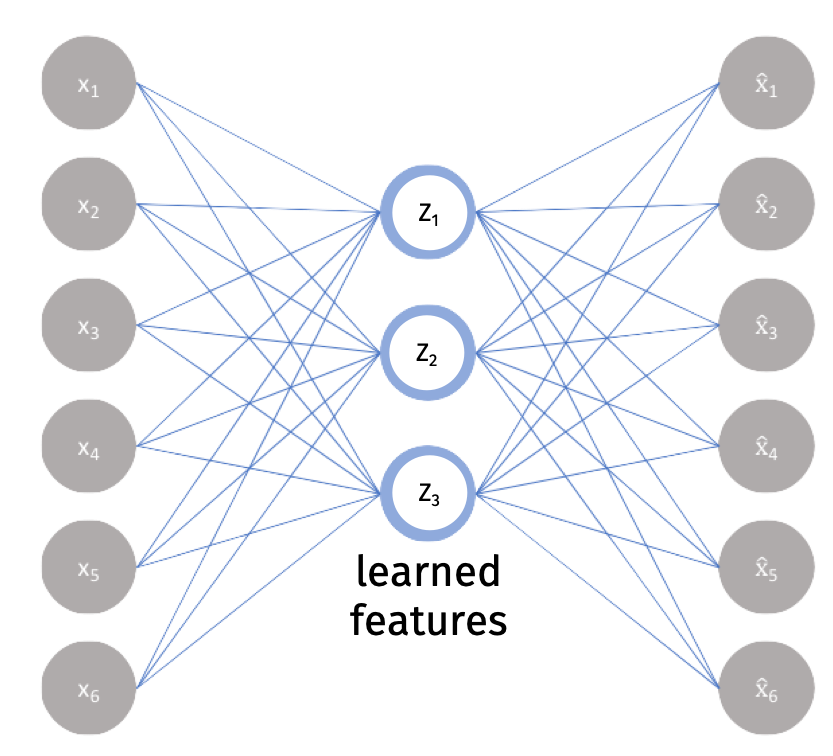
\includegraphics[width=.4\textwidth]{bottleneck.png}
	\end{center}
\vspace{-1.5em}
\textbf{Definitions:}
\begin{itemize}
	\item Let $\mathcal{A}$ be our original data space. E.g. $\mathcal{A} = \R^d$ for some dimension $d$. 
	
	\item Let $\mathcal{S}$ be the set of all data examples which \emph{could} be the output of our autoencoder $f$. We have that $\mathcal{S} \subset \mathcal{A}$. Formally,  $\mathcal{S} = \{\vec{y} \in \R^d: \vec{y} = f(\vec{x}) \text{ for some } \vec{x}\in \R^d\}$.
\end{itemize}

\end{frame}

\begin{frame}
	\small
	\frametitle{autoencoders learn compressed representations}
	\begin{center}
		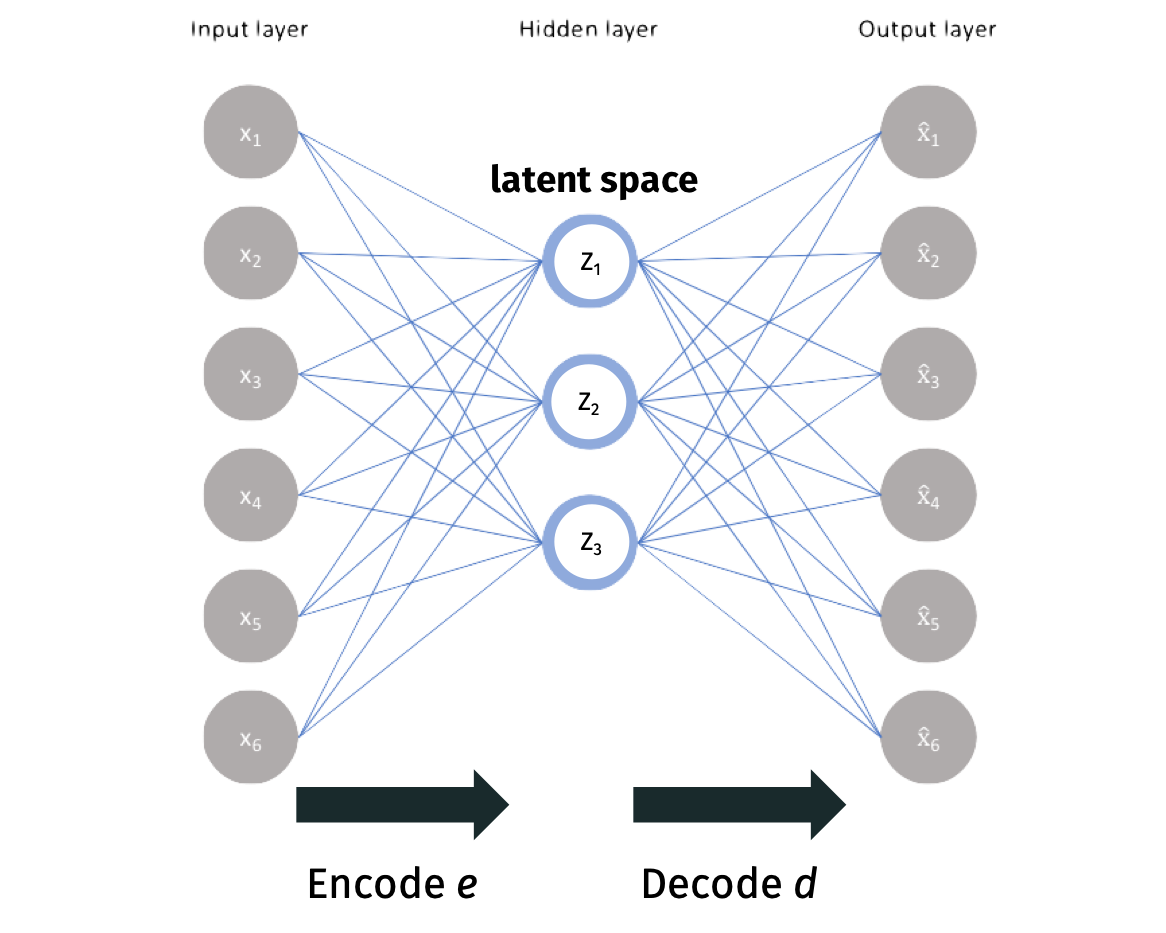
\includegraphics[width=.5\textwidth]{labeled_bottleneck.png}
	\end{center}
\vspace{-1em}
	Consider $128\times 128 \times 3$ images with pixels values in $0, 1 \ldots, 255$. How many unqique images are there in $\mathcal{A}$?\vspace{2em}
	
	Suppose $\vec{z}$ holds $k$ values between in $0,.1,.2,\ldots, 1$. Roughly how many unique images are there in $\mathcal{S}$?
\end{frame}

\begin{frame}
	\frametitle{autoencoders learn compressed representations}
	So, any autoencoder can only represent a \emph{tiny fraction} of all possible images. This is a \emph{good thing}.
	\begin{center}
	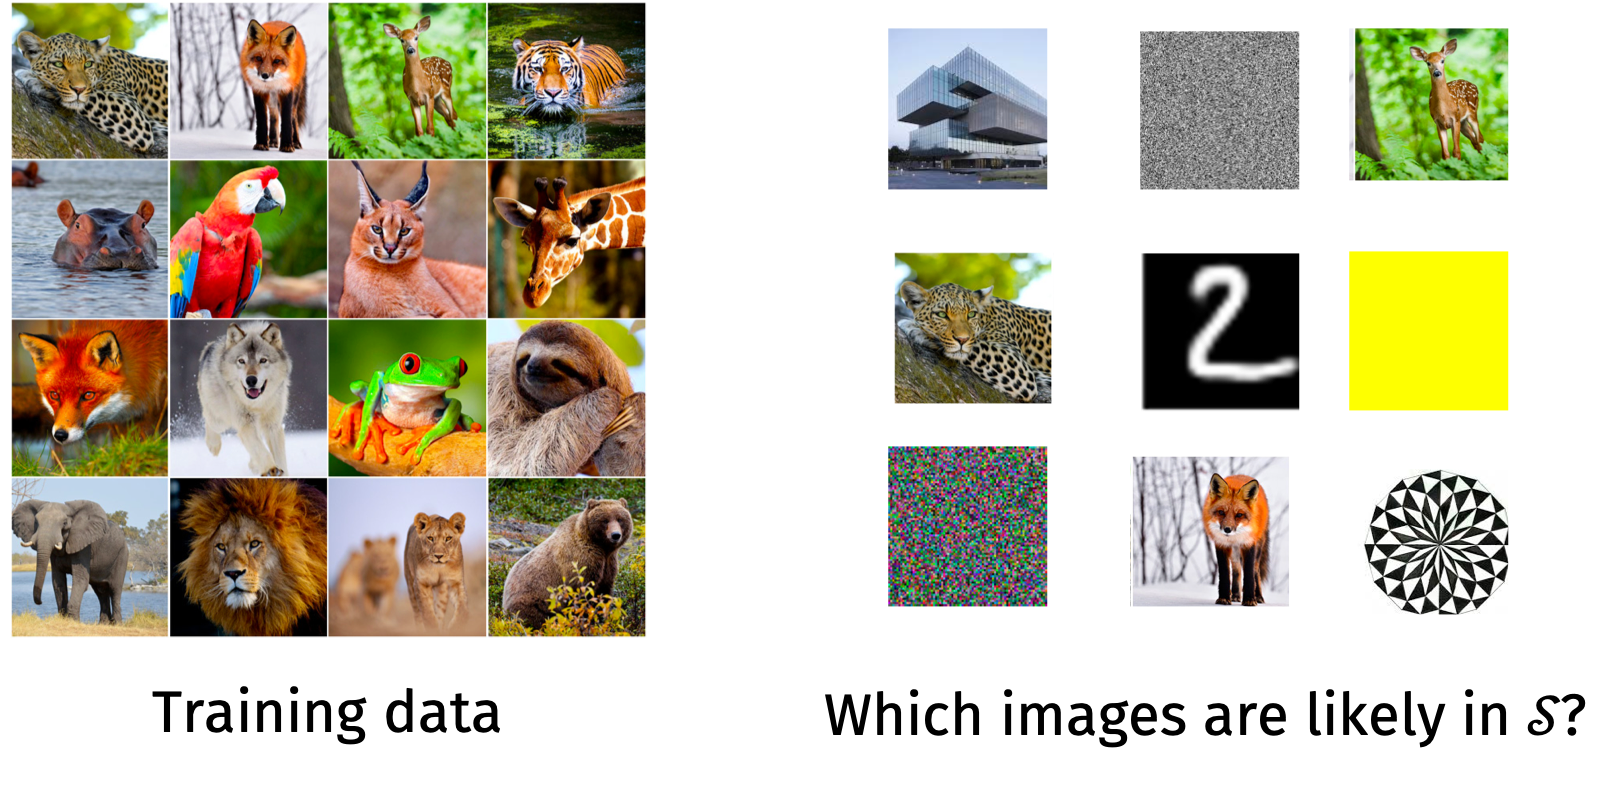
\includegraphics[width=.8\textwidth]{encoder_think.png}
	\end{center}
	
\end{frame}

\begin{frame}
	\frametitle{autoencoders learn compressed representations}
	\begin{center}
		$\mathcal{S} = \{\vec{y} \in \R^d: \vec{y} = f(\vec{x}) \text{ for some } \vec{x}\in \R^d\}$
		
		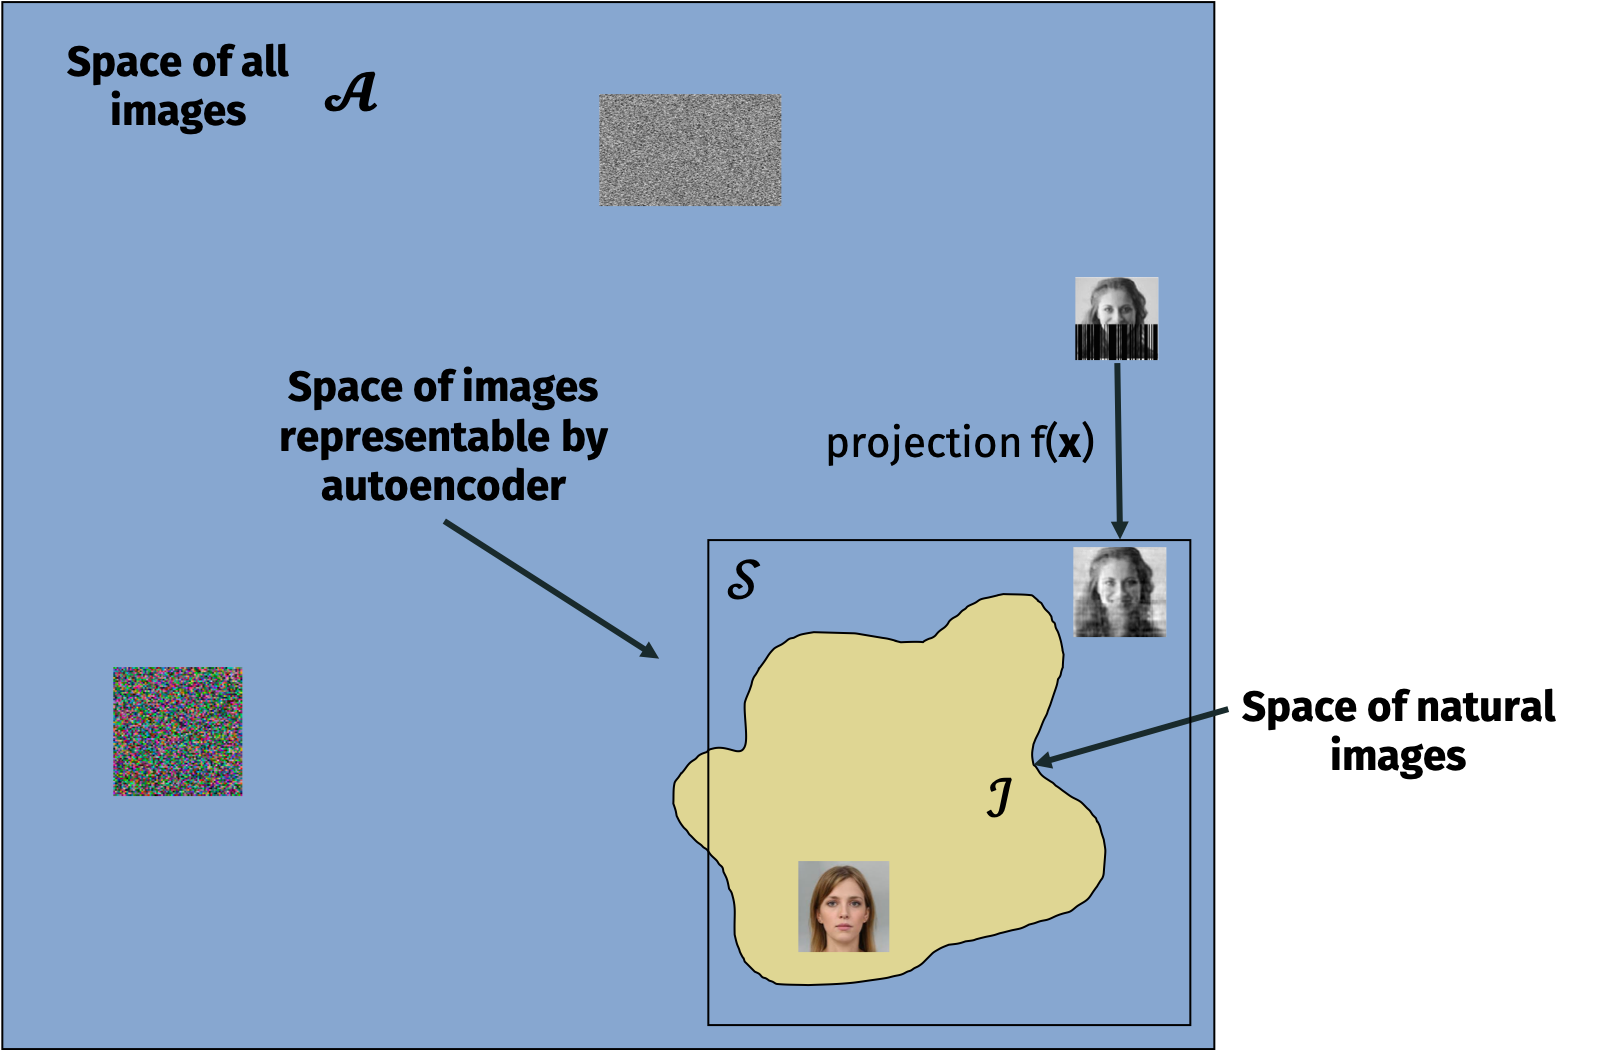
\includegraphics[width=.7\textwidth]{autoencoder_cartoon.png}
	\end{center}
	For a good (accurate, small bottleneck) autoencoder, $\mathcal{S}$ will closely approximate $\mathcal{I}$. Both will be much smaller than $\mathcal{A}$. 
\end{frame}

\begin{frame}
	\frametitle{autoencoders learn compressed representations}
	\begin{center}
		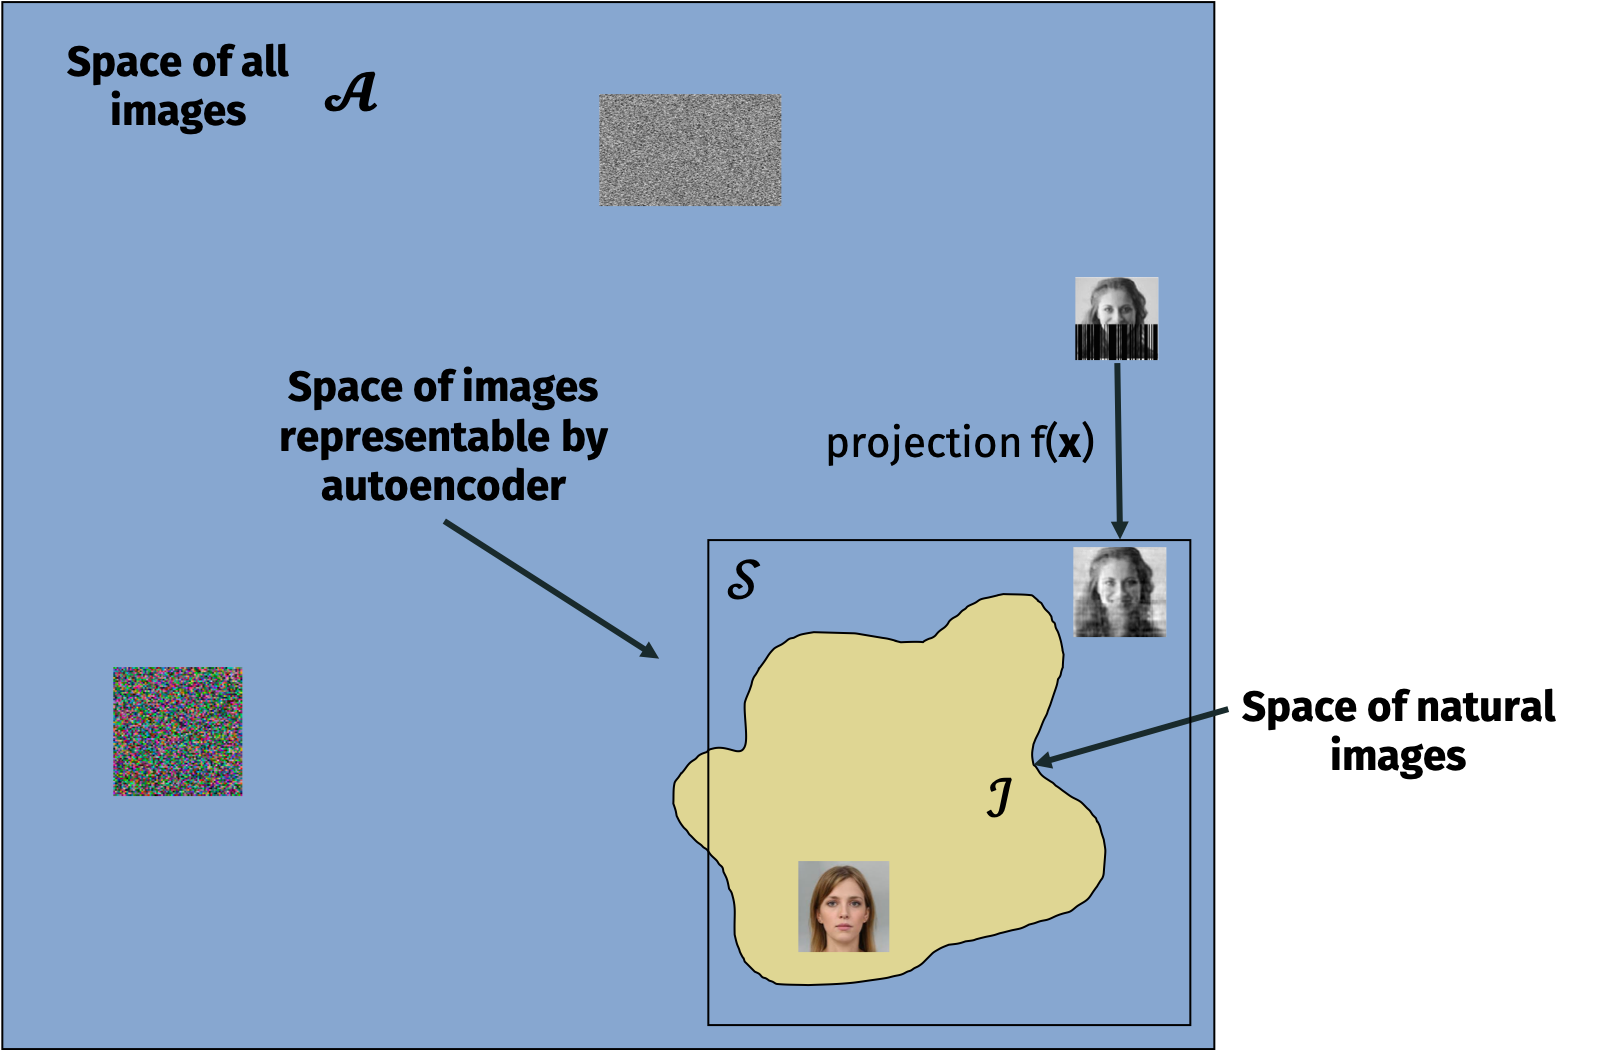
\includegraphics[width=.8\textwidth]{autoencoder_cartoon.png}
	\end{center}
	$f(\vec{x})$ projects an image $\vec{x}$ closer to the space of natural images.
\end{frame}

\begin{frame}
	\frametitle{autoencoders for data generation}
	Suppose we want to generate a random natural image. How might we do that?
	

	\begin{itemize}
		\item \textbf{Option 1}: Draw each pixel in $\vec{x}$ value uniformly at random. Draws a random image from $\mathcal{A}$.
			\begin{center}
		
\includegraphics[width=.3\textwidth]{noise.png}
			\end{center}
		
		\item \textbf{Option 2}: Draws $\vec{x}$ randomly image from $\mathcal{S}$. 
				\begin{center}
		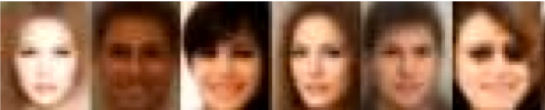
\includegraphics[width=.3\textwidth]{faces.png}
			\end{center}
	\end{itemize}

How do we randomly select an image from $\mathcal{S}$? 
\end{frame}

\begin{frame}
	\frametitle{autoencoders for data generation}
	\small
	How do we randomly select an image $\vec{x}$ from $\mathcal{S}$? 
	\vspace{-.5em}
	\begin{center}
		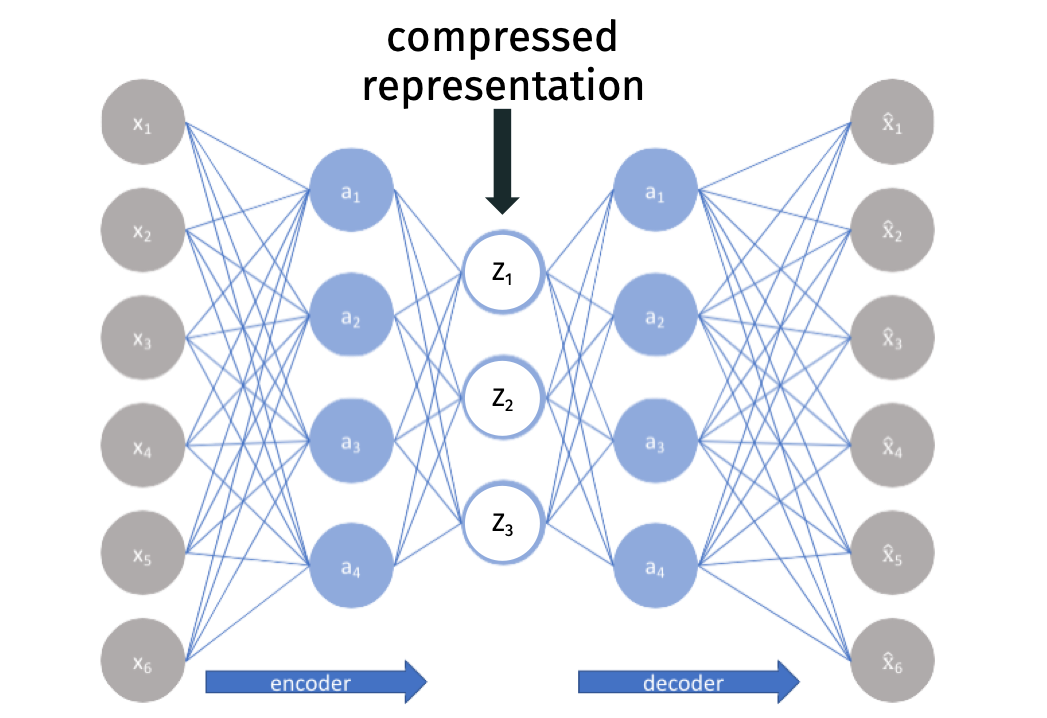
\includegraphics[width=.5\textwidth]{compressed_rep.png}
	\end{center}
	\vspace{-.5em}
	Randomly select code $\vec{z}$, then set $\vec{x} = e(\vec{z}).$\footnote{Lots of details to think about here. In reality, people use ``variational autoencoders'' (VAEs), which are a  natural modification of AEs.}
\end{frame}

\begin{frame}
	\frametitle{autoencoders for data generation}
	\small
	\begin{center}
		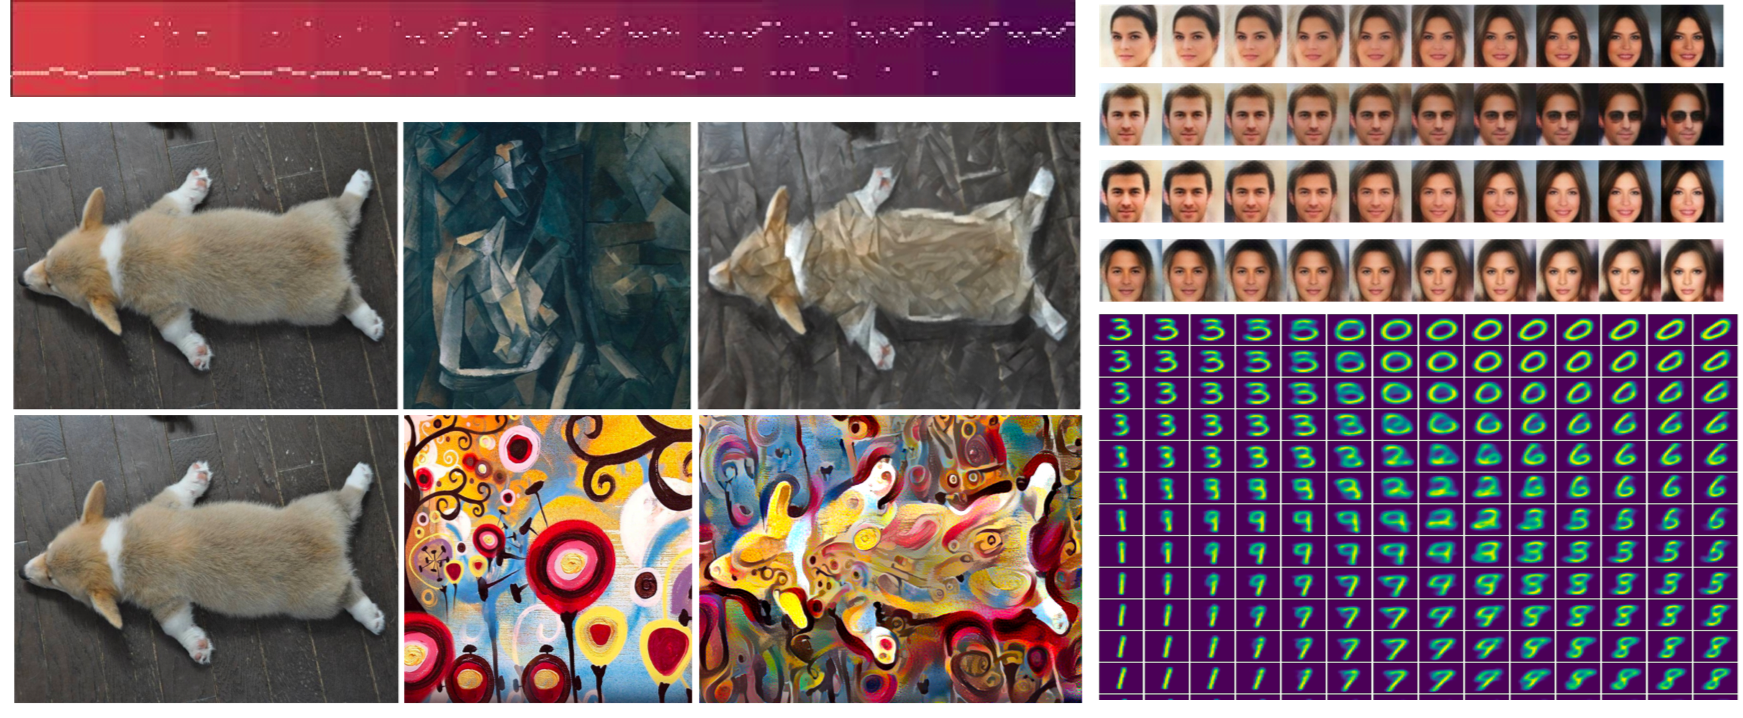
\includegraphics[width=\textwidth]{data_generation.png}
	\end{center}
	\textbf{\alert{Generative models}} are a growing area of machine learning, drive by a lot of interesting new ideas. \emph{Generative Adversarial Networks} in particular are now a major competitor with \emph{variational autoencoders}.
\end{frame}

\begin{frame}
	\frametitle{principal component analysis}
	\textbf{Remainder of lecture:} Deeper dive into understanding a simple, but powerful autoencoder architecture. Specifically we will learn about \textbf{\alert{principal component analysis (PCA)}}  as a type of autoencoder.
	
	PCA is the ``linear regression" of unsupervised learning: often the go-to baseline method for feature extraction and dimensionality reduction.
	
	Very important outside machine learning as well.
\end{frame}

\begin{frame}
	\frametitle{principal component analysis}
	\small
	Consider the simplest possible autoencoder:
	\begin{center}
		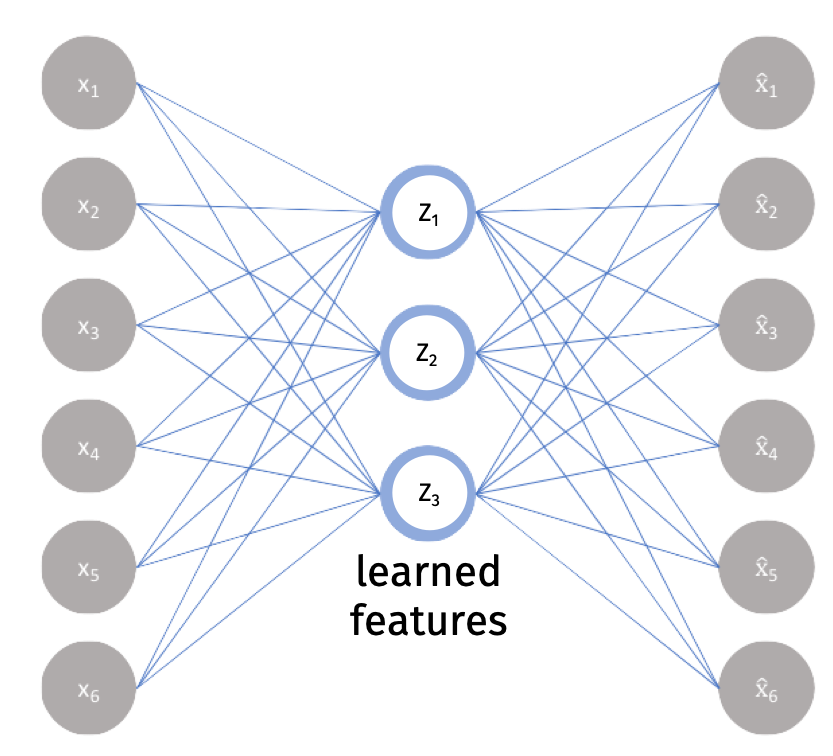
\includegraphics[width=.5\textwidth]{bottleneck.png}
	\end{center}
	\begin{itemize}
		\item One hidden layer. No non-linearity. No biases.
		\item Latent space of dimension $k$. 
		\item Weight matrices are $\bv{W}_1\in \R^{d\times k}$ and $\bv{W}_2\in \R^{k\times d}$. 
	\end{itemize}
\end{frame}

\begin{frame}
	\frametitle{principal component analysis}
	Given input $\vec{x}\in \R^d$, what is $f(\vec{x})$ expressed in linear algebraic terms?
		\begin{center}
		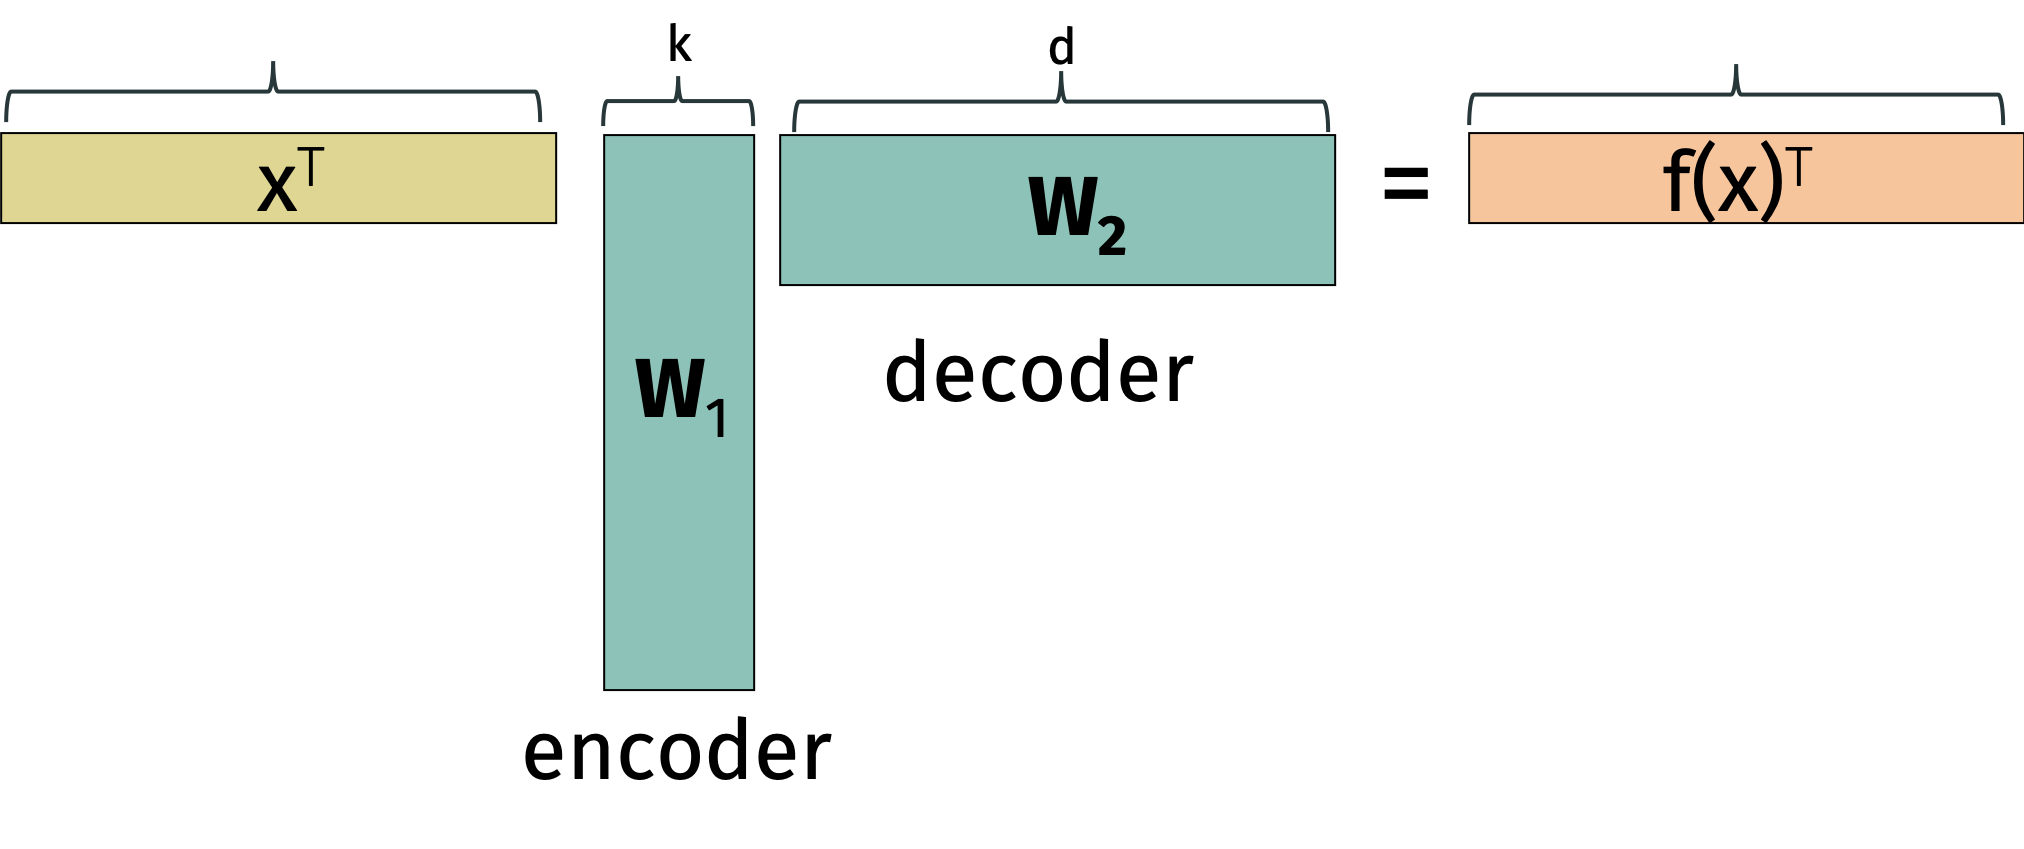
\includegraphics[width=.8\textwidth]{auto_alg.png}
	\end{center}
\begin{align*}
	f(\vec{x})^T = \vec{x}^T\bv{W}_1\bv{W}_2
\end{align*}
\end{frame}
\begin{frame}
	\frametitle{principal component analysis}
	\begin{center}
		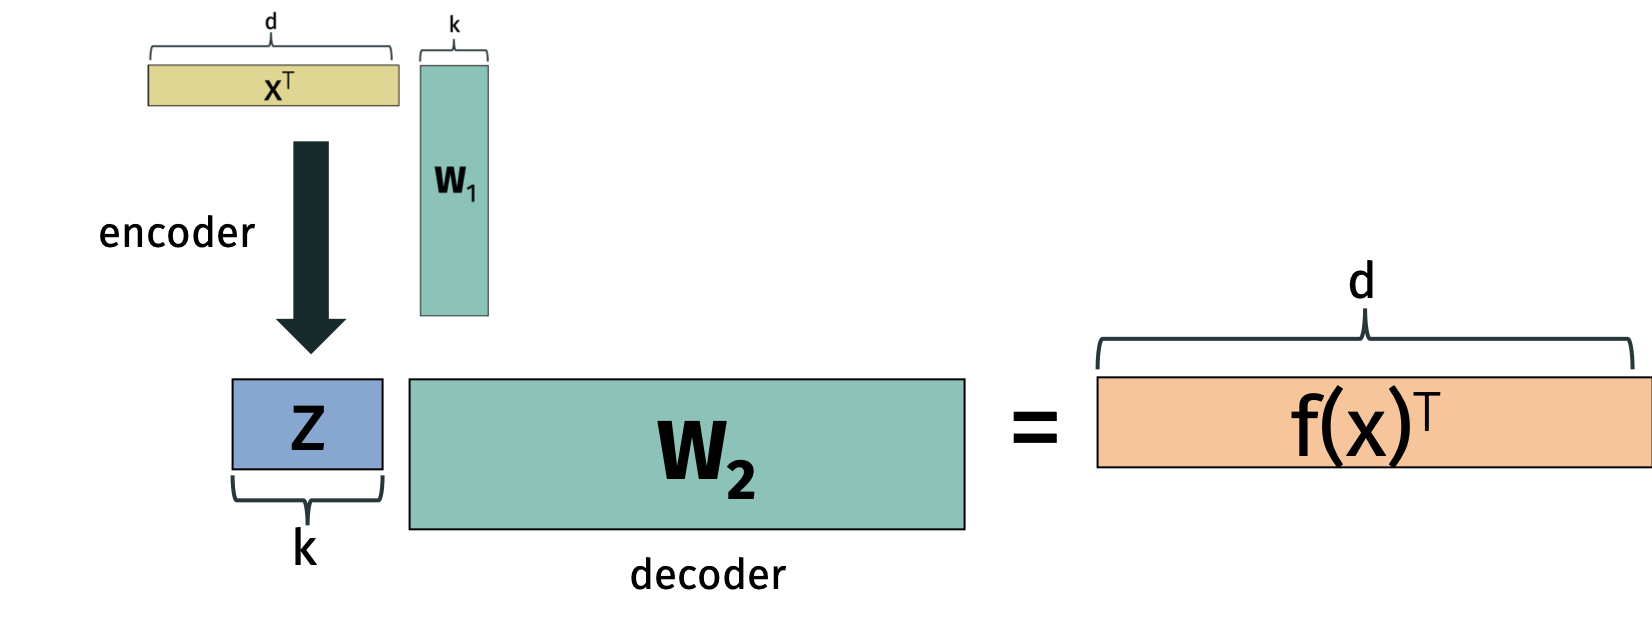
\includegraphics[width=.8\textwidth]{enc_dec.png}
	\end{center}
	\begin{center}
		\textbf{Encoder:} $e(\vec{x}) = \vec{x}^T \bv{W}_1$. \hspace{2em} \textbf{Decoder:} $d(\vec{z}) = \vec{z}\bv{W}_2$
	\end{center}
\end{frame}

\begin{frame}
	\frametitle{principal component analysis}
	Given training data set $\vec{x}_1, \ldots, \vec{x}_n$, let $\bv{X}$ denote our data matrix. Let  $\tilde{\bv{X}} = \bv{X}\bv{W}_1\bv{W}_2$.
	\begin{center}
		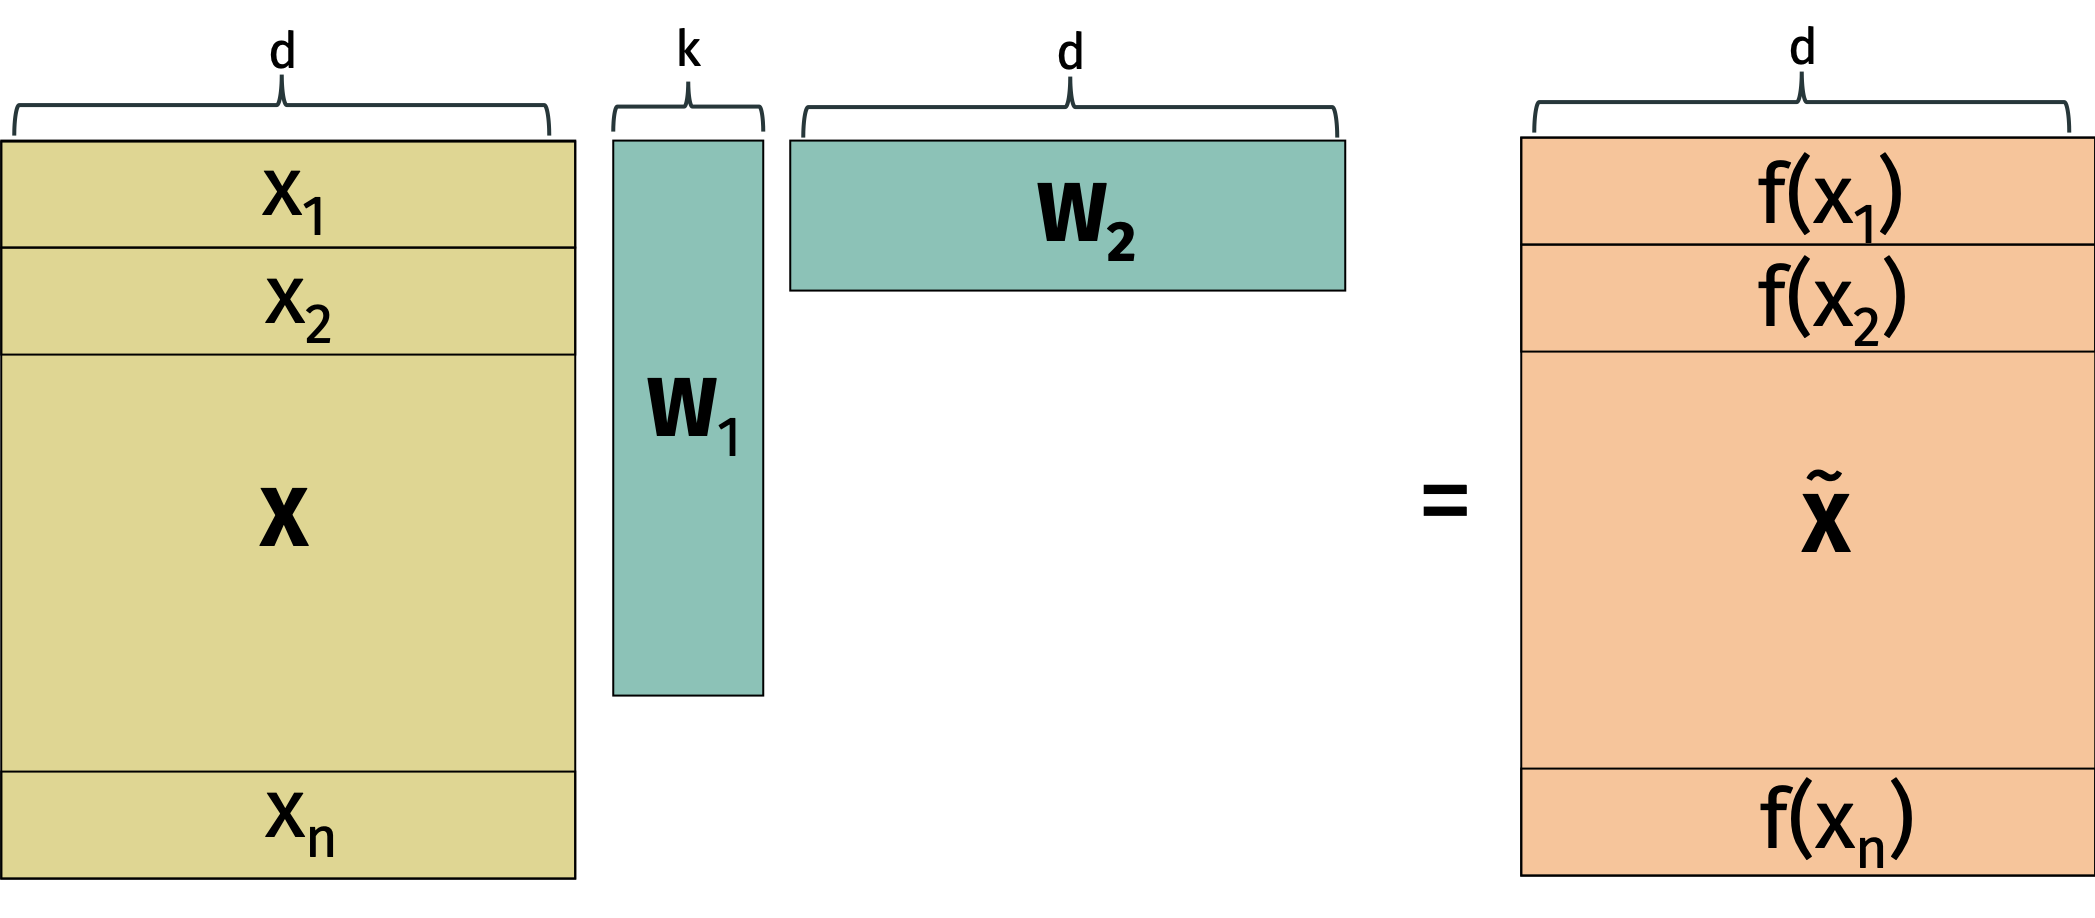
\includegraphics[width=.8\textwidth]{auto_alg_agg.png}
	\end{center}
	\textbf{Goal of training autoencoder:} Learn weights (i.e. learn matrices $\bv{W}_1\bv{W}_2$) so that $\tilde{\bv{X}}$ is as close to $\bv{X}$ as possible. 
\end{frame}

\begin{frame}
	\frametitle{frobenius norm}
	\textbf{Natural squared autoencoder loss:} Minimize $L(\bv{X}, \tilde{\bv{X}})$ where:
	\begin{align*}
	L(\bv{X}, \tilde{\bv{X}}) &= \sum_{i=1}^n \|\vec{x}_i - f(\vec{x}_i)\|_2^2\\
	&= \sum_{i=1}^n \sum_{j=1}^d (\vec{x}_i[j] - f(\vec{x}_i)[j])^2\\
	&= \|\bv{X} - \tilde{\bv{X}}\|_F^2
	\end{align*}
	Recall that for a matrix $\bv{M}$, $\|\bv{M}\|_F^2$ is called the \emph{Frobenius norm}. $\|\bv{M}\|_F^2 = \sum_{i,j} \bv{M}_{i,j}^2$.
	
	\textbf{Question:} How should we find $\bv{W}_1, \bv{W}_2$ to minimize $\|\bv{X} - \tilde{\bv{X}}\|_F^2 = \|\bv{X} - \bv{X}\bv{W}_1\bv{W}_2\|_F^2$?
\end{frame}

\begin{frame}
	\frametitle{low-rank approximation}
	\small
	\textbf{Recall:} \vspace{-.5em}
	
	\begin{itemize}
		\item The columns of a matrix with \emph{column rank} $k$ can all be written as linear combinations of just $k$ columns.\vspace{-.25em}
		\item The rows of a matrix with \emph{row rank} $k$ can all be written as linear combinations of $k$ rows.\vspace{-.25em}
		\item  Column rank = row rank = \textbf{rank}.\vspace{-.25em}
	\end{itemize} 
\vspace{-1em}
	\begin{center}
		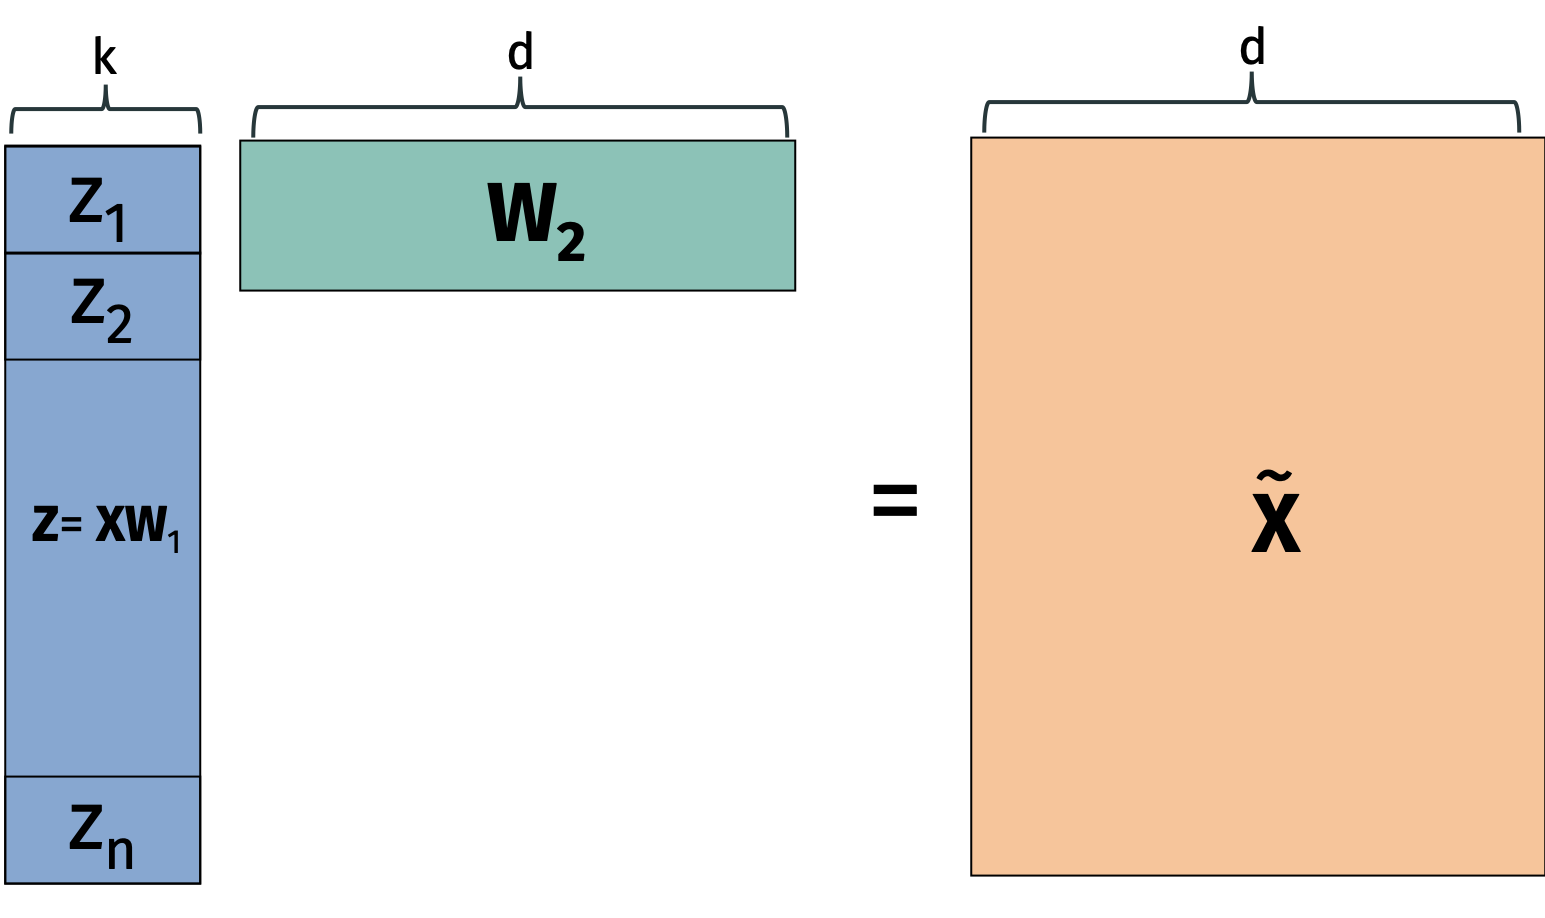
\includegraphics[width=.6\textwidth]{lowranktilde.png}
		
		$\tilde{\bv{X}}$ is a \alert{\textbf{low-rank matrix}} since it has rank $k$ for $k \ll d$.
	\end{center}
\end{frame}

\begin{frame}
	\frametitle{low-rank approximation}
	Principal component analysis is the task of finding $\bv{W}_1$, $\bv{W}_2$, which amounts to finding a rank $k$ matrix $\tilde{\bv{X}}$ which approximates the data matrix $\bv{X}$ as closely as possible. 
	
	In general, $\bv{X}$ will have rank $d$. 
\end{frame}

\begin{frame}
	\frametitle{singular value decomposition}
	\small
	\emph{Any} matrix $\bv{X}$ can be written:
	\begin{center}
		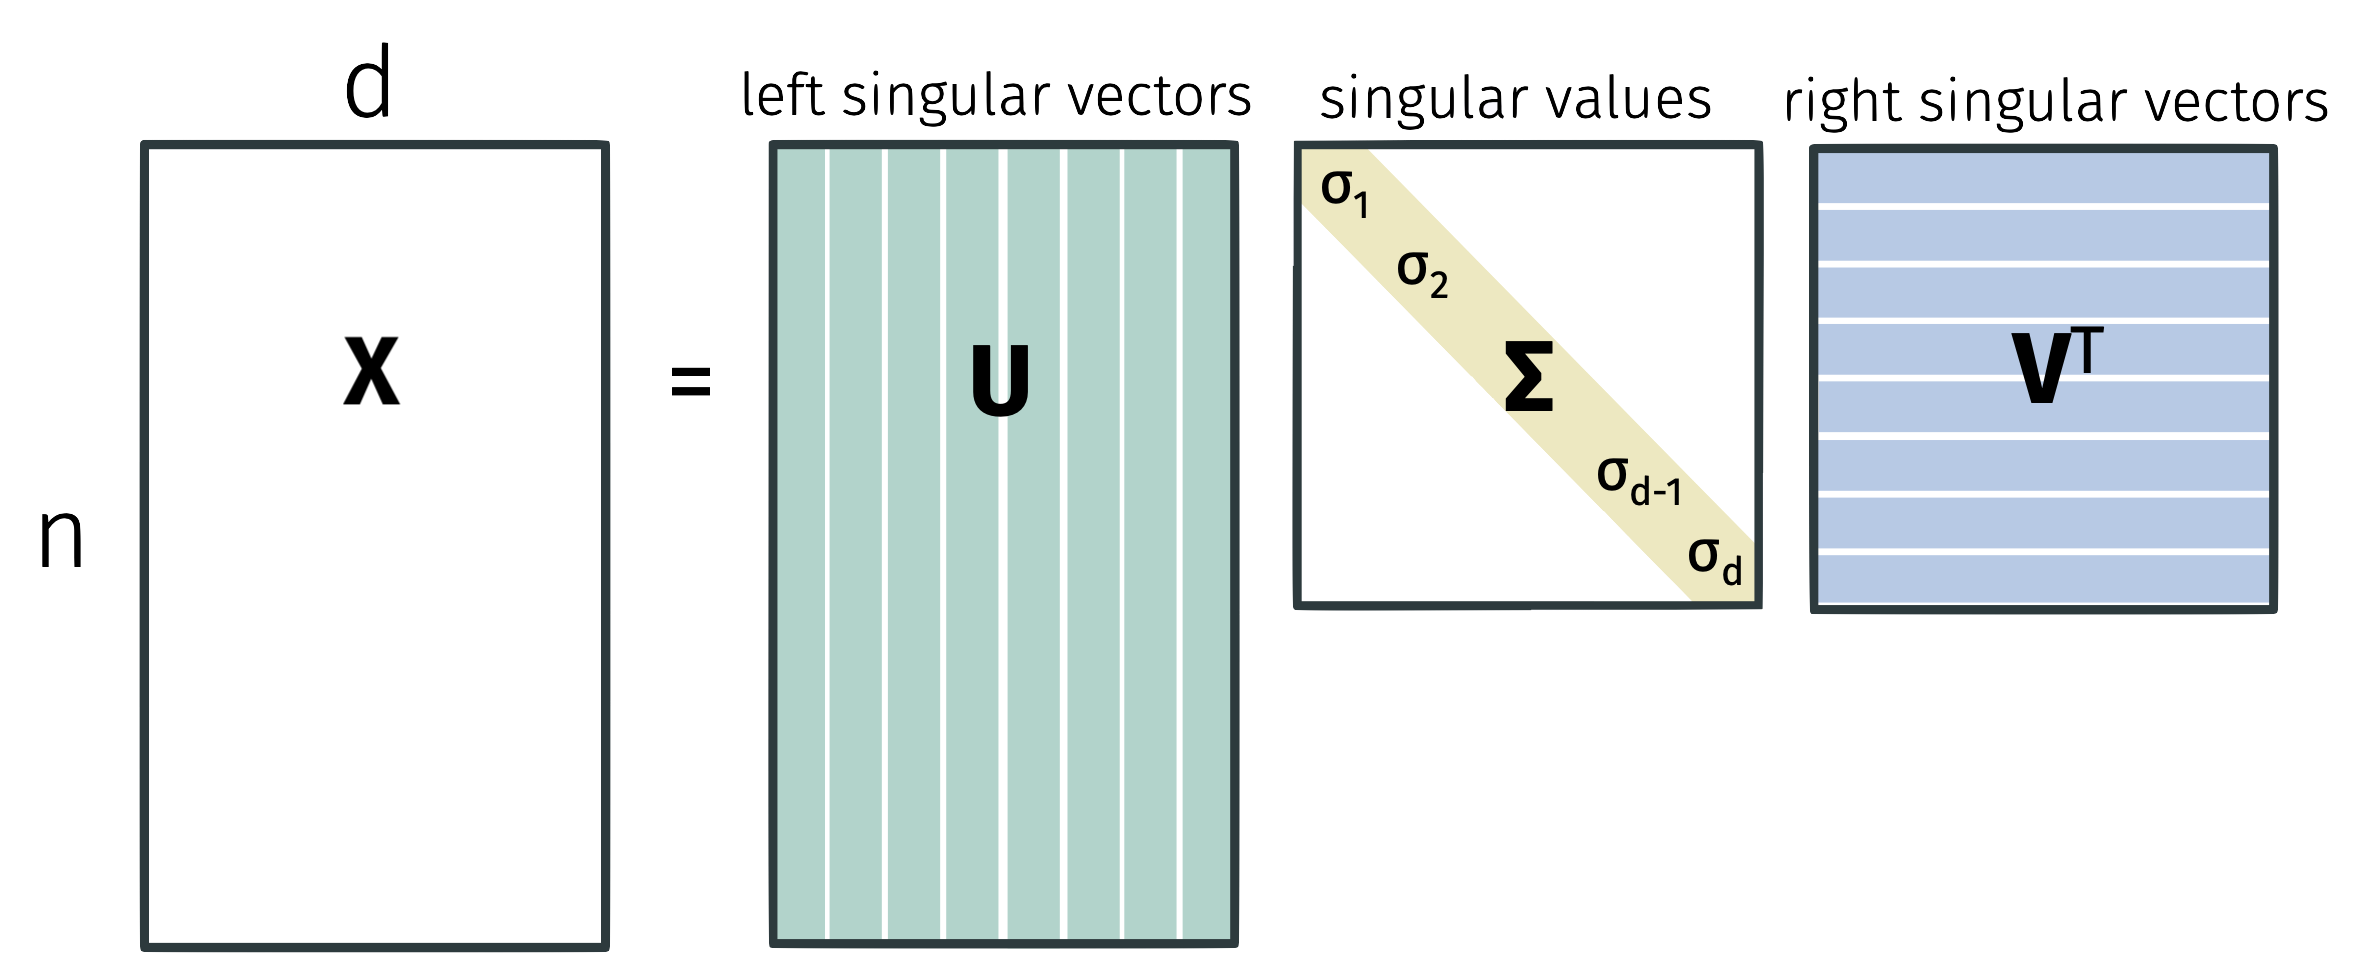
\includegraphics[width=.9\textwidth]{svd.png}
	\end{center} 
	Where $\bv{U}^T\bv{U} = \bv{I}$,  $\bv{V}^T\bv{V} = \bv{I}$, and $\sigma_1 \geq \sigma_2 \geq \ldots \sigma_d \geq 0$. I.e. $\bv{U}$ and $\bv{V}$ are \emph{orthogonal matrices}.
	\begin{center}
		\normalsize This is called the \textbf{singular value decomposition.}
	\end{center}
Can be computed in $O(nd^2)$ time (faster with approximation algos).
\end{frame}

\begin{frame}
	\frametitle{orthogonal matrices}
	Let $\bv{u}_1, \ldots, \bv{u}_n \in \R^n$ denote the columns of $\bv{U}$. I.e. the top left singular vectors of $\bv{X}$. 
		\begin{center}
		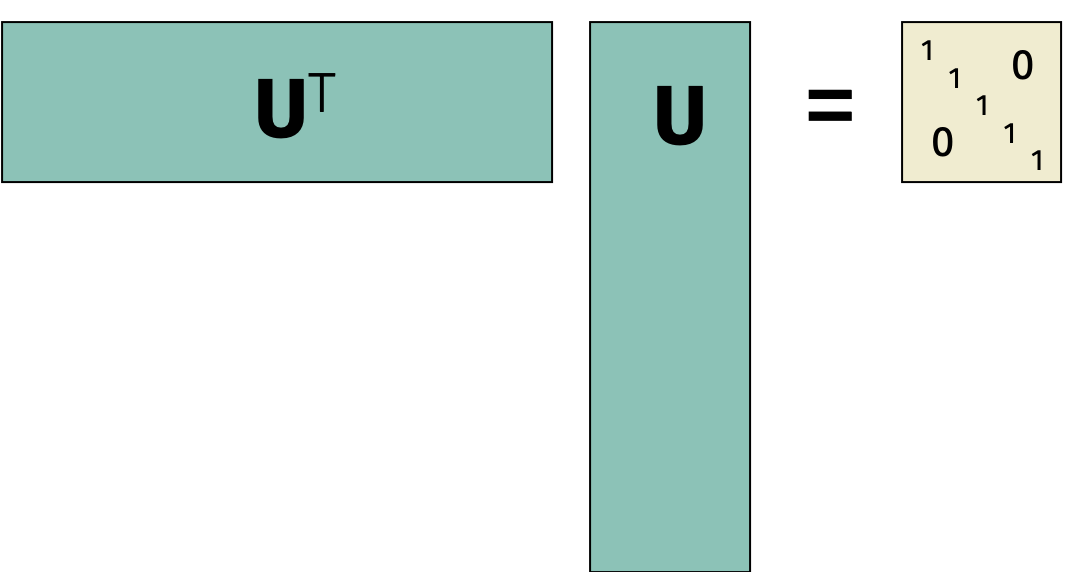
\includegraphics[width=.5\textwidth]{orthogonal.png}
	\end{center}
\begin{center}
	$\|u_i\|_2^2 = $ \hspace{8em} $\bv{u}_i^T\bv{u}_j = $
\end{center}
	
\end{frame}

\begin{frame}[t]
	\frametitle{singular value decomposition}
	Can read off optimal low-rank approximations from the SVD:
	\begin{center}
		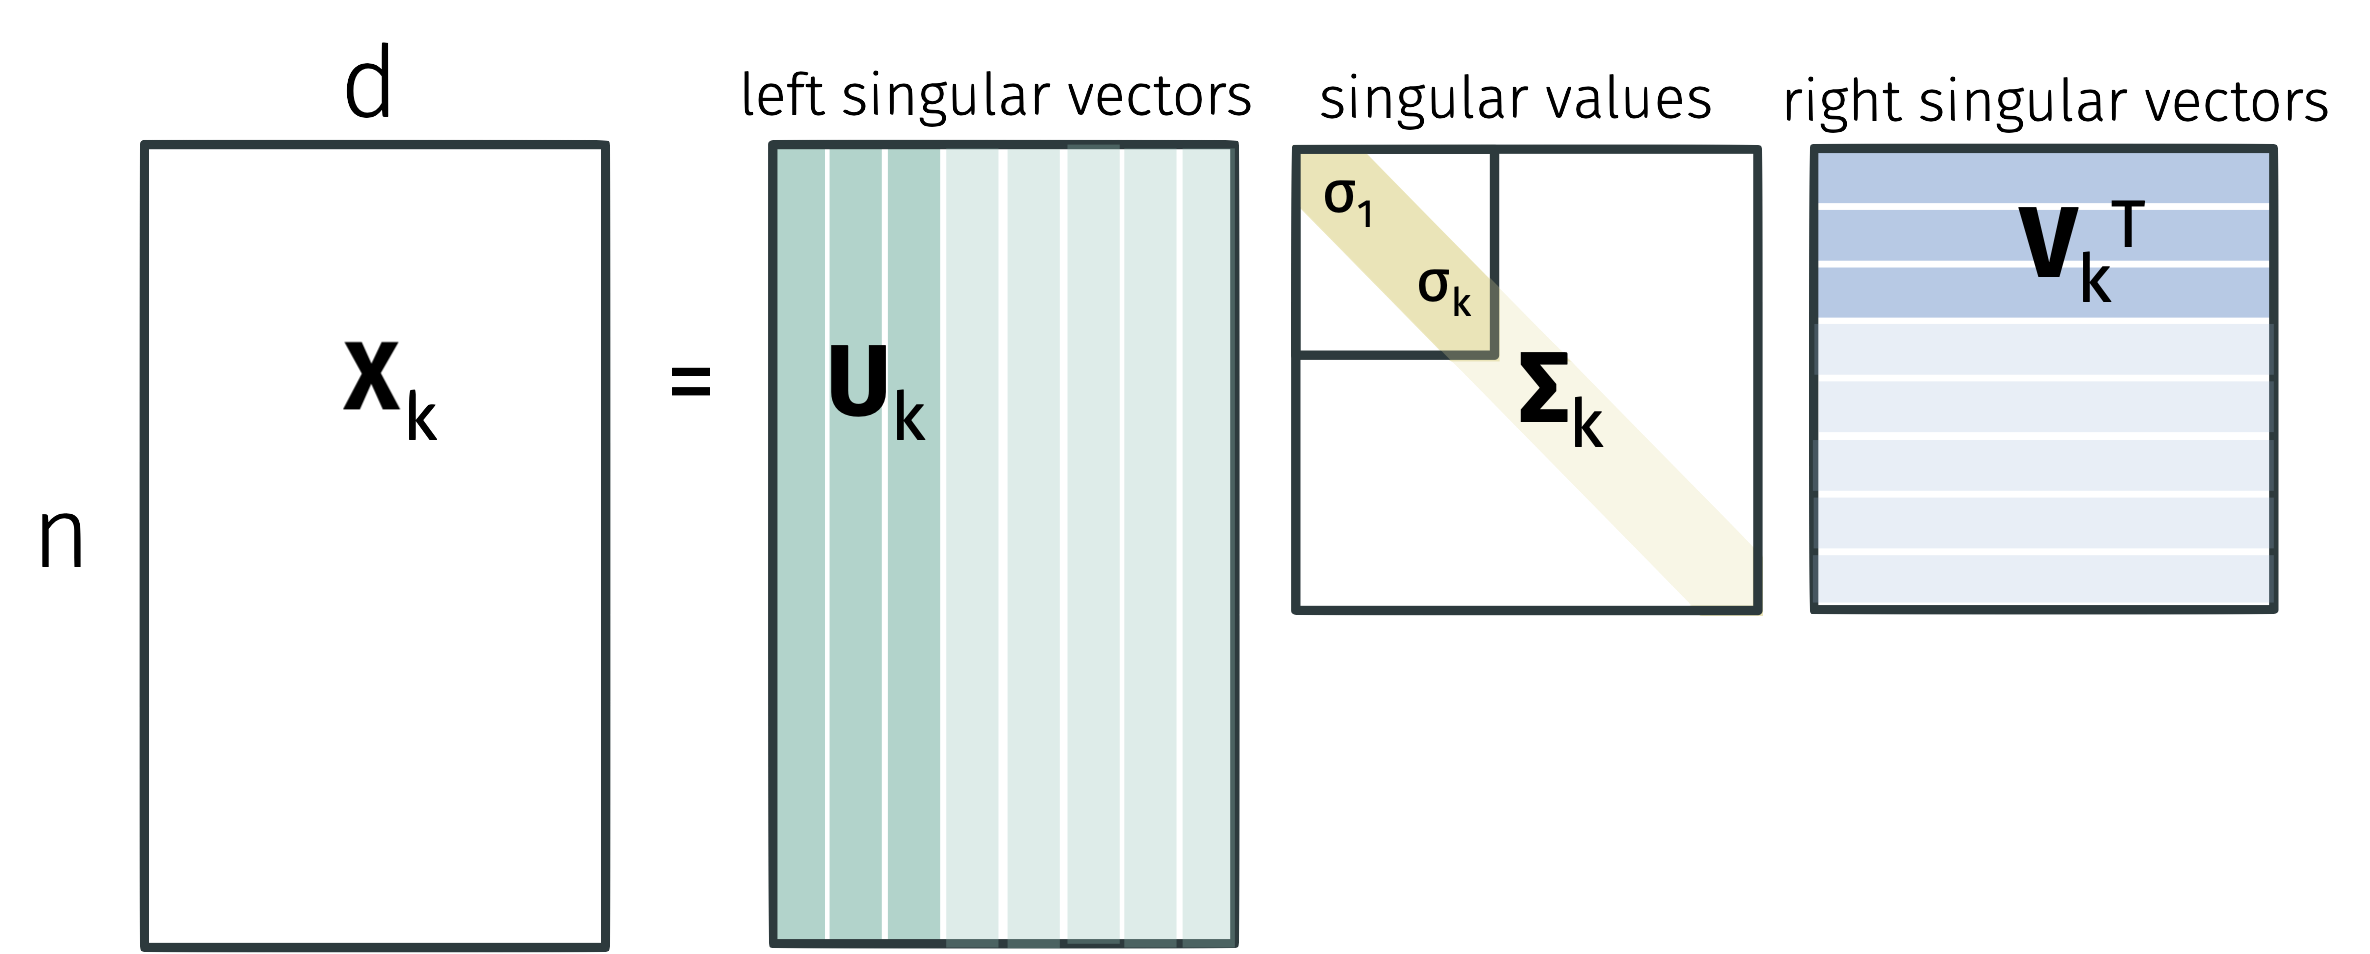
\includegraphics[width=.9\textwidth]{svdk.png}
	\end{center} 
	\textbf{Eckart–Young–Mirsky Theorem:} For any $k \leq d$, $\bv{X}_k = \bv{U}_k\bs{\Sigma}_k\bv{V}_k^T$ is the optimal $k$ rank approximation to $\bv{X}$:
	\begin{align*}
	\bv{X}_k = 	\argmin_{\tilde{\bv{X}} \text{ with rank $\leq k$} } \|\bv{X} - \tilde{\bv{X}}\|_F^2.
	\end{align*}
\end{frame}

\begin{frame}[t]
	\frametitle{singular value decomposition}
	\textbf{Claim:} $\bv{X}_k = \bv{U}_k\bs{\Sigma}_k\bv{V}_k^T = \bv{X}\bv{V}_k\bv{V}_k^T$.
	\vspace{15em}
	
	So for a model with $k$ hidden variables, we obtain an \emph{optimal} autoencoder by setting $\bv{W}_1 =\bv{V}_k$, $\bv{W}_2 = \bv{V}_k^T$. $f(\vec{x}) = \vec{x}\bv{V}_k\bv{V}_k^T$.
\end{frame}

\begin{frame}[t]
	\frametitle{principal component analysis}
	\begin{center}
		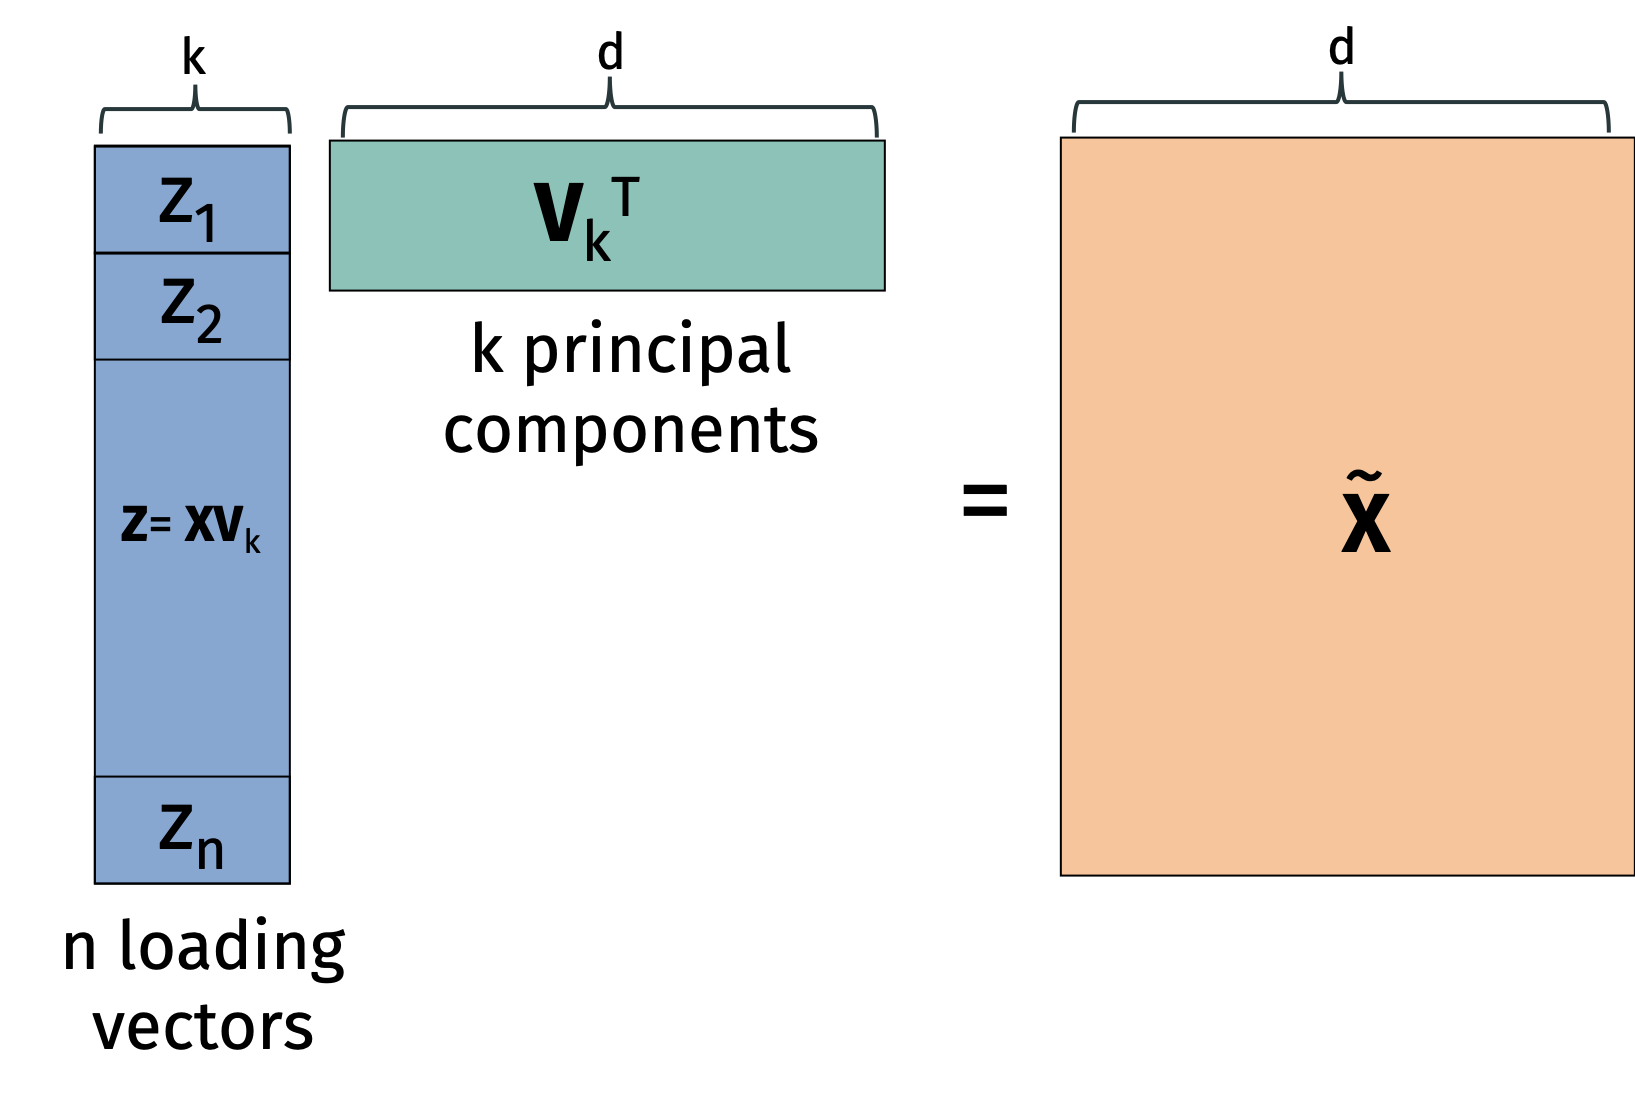
\includegraphics[width=.9\textwidth]{pca.png}
	\end{center} 
	
	To be continued...
\end{frame}

%\begin{frame}
%	\frametitle{image segmentation}
%	\textbf{Goal:} Learn mask which separates image pixels by what object (foreground or background) that they belong to.
%	\begin{center}
%		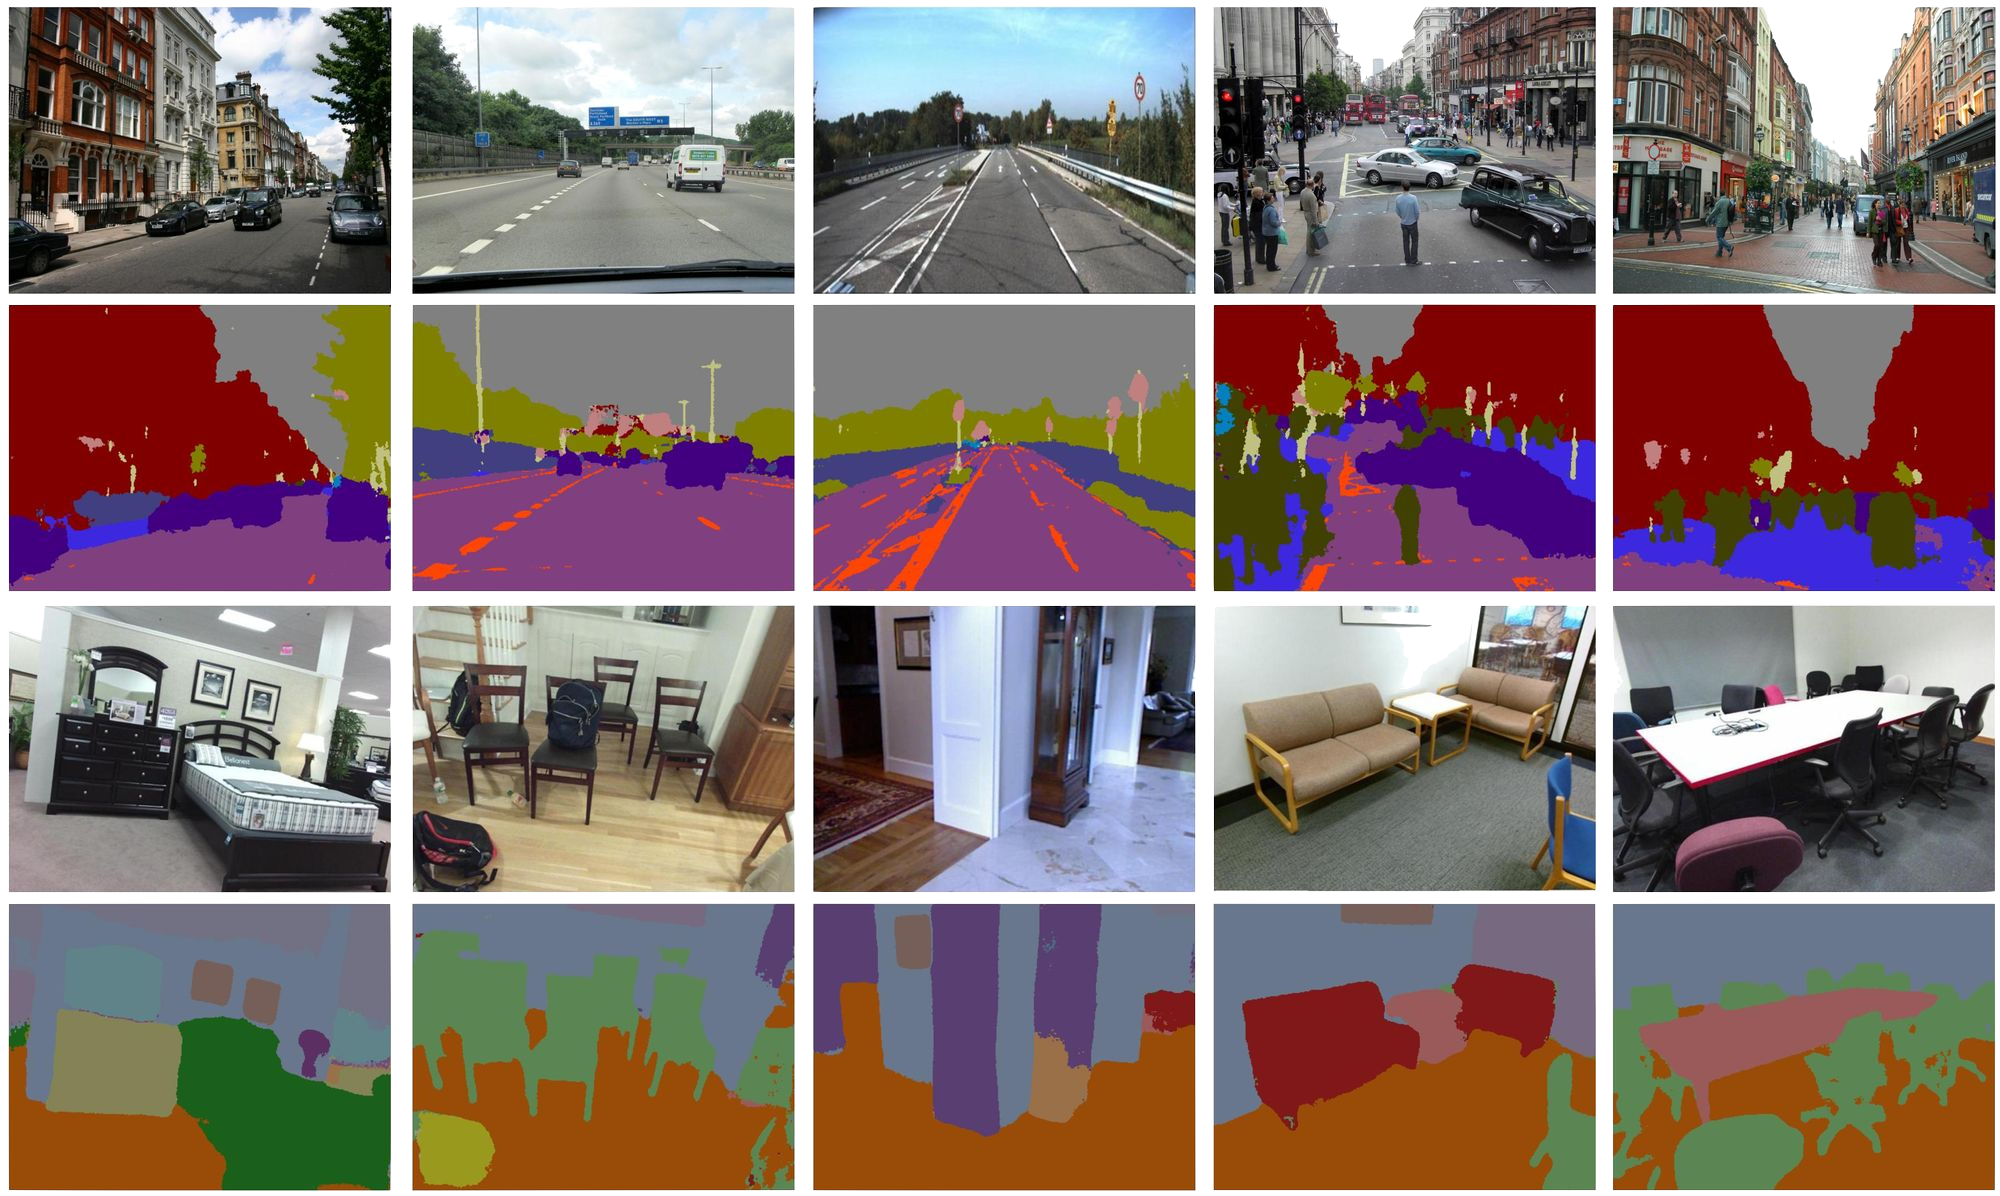
\includegraphics[width=.8\textwidth]{segment.png}
%	\end{center}
%	First step in \emph{multi-objects classification} and \emph{scene understanding}. Harder than classifying single objects.
%\end{frame}
%
%\begin{frame}
%	\frametitle{autoencoders for image segmentation}
%	\textbf{Change in design:} Input is image $\vec{x}$, output is image $\vec{m}$ that has the same size as $\vec{x}$, but each pixel value is a label for a segmented region.
%	\begin{center}
%		\includegraphics[width=.8\textwidth]{deepseg.png}
%	\end{center}
%	Now our training process is actually \emph{supervised}, but uses the same structure as an autoencoder.
%\end{frame}

\end{document} 



